\documentclass{article}

\usepackage{neurips_2026}

\usepackage[utf8]{inputenc}
\usepackage[T2A,T1]{fontenc}
\usepackage[english,russian]{babel}
\usepackage{hyperref}
\usepackage{url}
\usepackage{booktabs}
\usepackage{amsfonts}
\usepackage{amsmath}
\usepackage{nicefrac}
\usepackage{microtype}
\usepackage{xcolor}
\usepackage{graphicx}
\usepackage{array}
\usepackage{enumitem}
\usepackage{placeins}
\usepackage{tikz}
\usetikzlibrary{arrows.meta,positioning}

\newcommand{\method}[1]{\texttt{#1}}

\title{Q/R/M/C: измерительный фреймворк стадийной декомпозиции для навигации на основе памяти и минимальная коллективная семантическая память}

%\author{%
%  Anonymous Authors \\
%  Anonymous Institution \\
%  Anonymous Address \\
%  \texttt{anonymous@anonymous.edu} \\
%}

\begin{document}

\maketitle

\begin{abstract}
\textbf{Постановка.} Метрики, учитывающие только итоговый успех, схлопывают качественно различные отказы навигации на основе памяти в один скаляр, скрывая, \emph{какая стадия} конвейера извлечения за них отвечает. В настоящей работе разрабатывается измерительный фреймворк, а не новый теоретический результат: стадийная декомпозиция Q/R/M/C (\textbf{Q}uery --- формирование запроса, \textbf{R}etrieval --- удовлетворение извлечения, \textbf{M}aterialization --- материализация цели, \textbf{C}ompletion --- завершение после извлечения) операционализирована так, что четыре условные частоты вычислимы непосредственно из стандартных журналов траекторий (определение~1; аргумент согласованности --- это цепное правило, и мы говорим об этом явно).
\textbf{Одноагентные измерения.} На 10-сидовом бенчмарке MiniGrid (FourRooms, LavaGapS7) и проверке переносимости на BabyAI фреймворк локализует бутылочные горлышки: восстановление после опасности ограничено извлечением (оракульное извлечение поднимает успех $0.39\to0.60$), возврат в целевую область ограничен нисходящими стадиями. Инспекция журналов уточняет атрибуцию: ранжирование кандидатов почти оптимально ($96.9\%$), тогда как генерация кандидатов отказывает в 91\% точек принятия решений --- предел накопления памяти, а не ранжирования.
\textbf{Многоагентные измерения.} На многоагентной развертке из 35{,}640 прогонов по четырем коммуникационным архитектурам (независимая, общая шина, центральный агрегатор, одноранговая рассылка при восьми каденциях $K{\in}\{1,2,4,8,16,32,48,64\}$, 40 сидов) смещение бутылочного горлышка (bottleneck shift) между звеньями M и C проявляется непосредственно как отрицательная внутрикаденционная корреляция с пиком при $K{=}4$ (Пирсон $-0.61$); среднее время до успеха имеет внутренний минимум при $K{=}8$. Оба знака наклона (эмпирическое утверждение~1) подтверждаются при $p<10^{-4}$; мы \emph{не} утверждаем существование внутреннего максимума условного произведения $\Phi$, для которого данные демонстрируют монотонный тренд к границе независимых агентов.
\textbf{Минимальная коллективная семантическая память.} Четыре архитектуры находятся в углах более богатого пространства проектных решений, задаваемого явными правилами \emph{слияния}, \emph{доверия} и \emph{устаревания} (staleness). Мы инстанцируем минимальную коллективную семантическую память --- слияние, взвешенное доверием, с устареванием по экспоненциальному затуханию давности поверх одноранговой рассылки --- и измеряем ее на той же шкале Q/R/M/C, демонстрируя, что она доминирует над лучшей одноранговой архитектурой с фиксированной каденцией по (M$\,\times\,$C) в сценарии дефицита. Это превращает <<коллективную семантическую память>> из программного заявления в инстанцированный артефакт, оцениваемый по тем же журналам.
\textbf{Область применимости.} Все эксперименты выполнены в сеточных субстратах (MiniGrid, BabyAI, кастомная сетка $12{\times}10$). Вклад работы --- протокол измерения и первый прототип; более богатые субстраты (Habitat, ProcTHOR, VMAS) --- предмет будущей работы.
\end{abstract}

\section{Введение}

\begin{figure}[t]
  \centering
  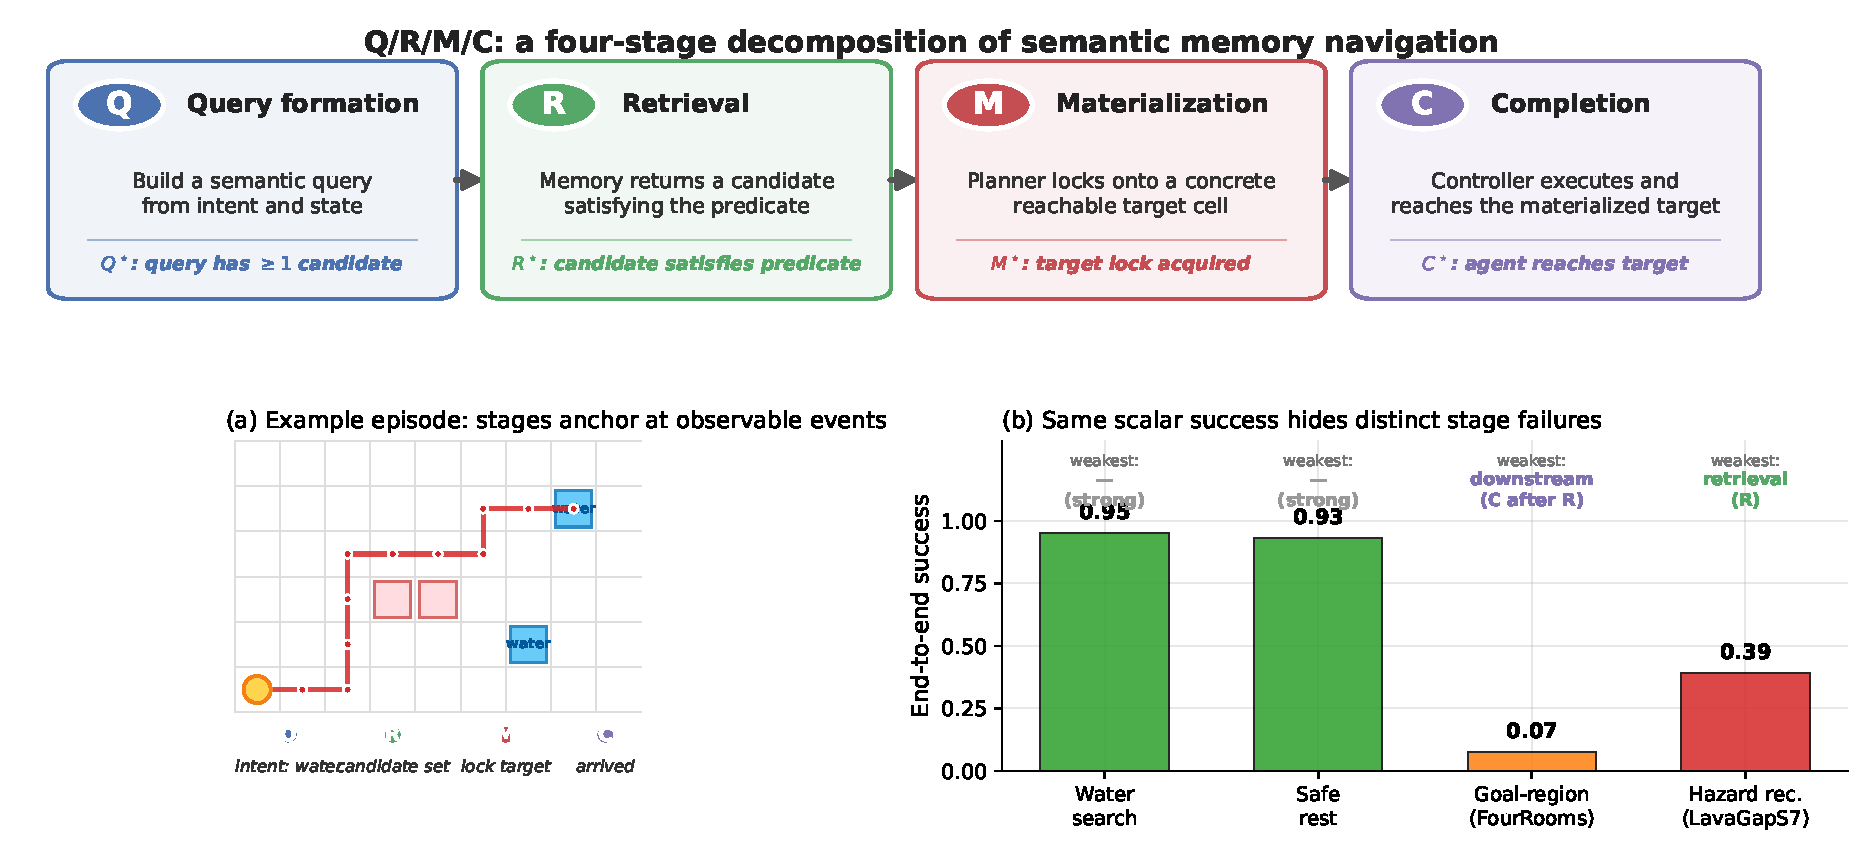
\includegraphics[width=\linewidth]{figures/fig_hero_qrmc.pdf}
  \caption{Q/R/M/C раскладывает один эпизод семантической навигации на четыре
  наблюдаемые стадии. \textbf{Сверху:} четыре стадии и их определения на уровне
  событий. \textbf{(a)} Успешный эпизод поиска воды закрепляется за
  одним событием на стадию, порождая логируемые помеченные звездочкой события
  $Q^\star, R^\star, M^\star, C^\star$. \textbf{(b)} Одна и та же скалярная
  сводка <<сквозного успеха>> маскирует качественно различные отказы
  на четырех одноагентных семействах задач: вода и отдых сильны;
  возврат в целевую область (FourRooms) ограничен нисходящими стадиями; восстановление
  после опасности (LavaGapS7) ограничено извлечением (оракульные интервенции, \S\ref{sec:oracle}).}
  \label{fig:hero}
\end{figure}

Классические навигационные бенчмарки часто предполагают, что агенту дана
явная координата пункта назначения или плотная награда за задачу. Многие практические
навигационные задачи устроены иначе: агент должен достичь места определенного
\emph{типа}, такого как безопасная зона отдыха, водоподобный ресурс,
выход для восстановления после опасности или область, ассоциированная с целью, заданного
семантическим паттерном, а не фиксированной точкой $(x, y)$. Следовательно, место
должно быть \emph{запомнено и извлечено по смыслу}. Такая
постановка открывает методологический вопрос: можем ли мы измерить, \emph{где}
ломается семантическая навигация на основе памяти, а не только \emph{ломается ли}
она вообще?

Мы отвечаем на этот вопрос четырехстадийным диагностическим фреймворком, который
применим как к одиночным агентам, так и к многоагентным коллективам.
Декомпозиция --- Q/R/M/C: формирование запроса (\textbf{Q}uery), удовлетворение
извлечения (\textbf{R}etrieval), материализация цели (\textbf{M}aterialization) и завершение
после извлечения (\textbf{C}ompletion). Декомпозиция факторизует по-эпизодное завершение
семантического пути и, при условном стадийно-марковском свойстве, ее факторы
оцениваемы из журналов траекторий (определение~1).
Остальная часть статьи развивает единый аргумент в трех частях.

\textbf{Одиночный агент.} Стадийная атрибуция нетривиальна.
Метрики только успеха схлопывают качественно различные отказы в
один скаляр. В 10-сидовом бенчмарке MiniGrid задачи воды и отдыха
сильны сквозным образом (успех 0.95, 0.93), но возврат в целевую область и
восстановление после опасности существенно сложнее, причем по \emph{разным
причинам}. Оракульные интервенции (oracle interventions) на стадиях показывают, что восстановление после опасности
ограничено извлечением (оракульное извлечение поднимает успех $0.39 \to 0.60$),
тогда как возврат в целевую область ограничен нисходящими стадиями (оракульное извлечение
спасает завершение семантического пути, не меняя сквозного успеха).
Инспекция собственных журналов фреймворка затем уточняет атрибуцию:
бутылочное горлышко извлечения --- это не \emph{ранжирование} кандидатов (точность
$96.9\%$, когда кандидаты существуют), а их \emph{генерация}: память
не содержит подходящих символов в 91\% точек принятия решений.
Одноагентное бутылочное горлышко --- это предел \emph{накопления памяти}:
свидетельства наблюдаются, но никогда не консолидируются в структуру, доступную для запросов.

\textbf{Многоагентный случай.} Консолидация приобретает скорость.
Когда $N$ агентов разделяют память через протокол рассылки с каденцией (cadence)
$K$, факторизация расширяется за счет увеличенных множеств обусловливания
(определение~2), и $K$ становится структурной осью: механически это
регулятор того, \emph{насколько быстро приватные памяти консолидируются
в коллективную}. Утверждение на уровне наклонов
(эмпирическое утверждение~1) предсказывает смещение бутылочного горлышка: при уменьшении $K$
$P(M^\star|R^\star)$ растет (более свежая память пиров обеспечивает
надежную фиксацию цели), а $P(C^\star|M^\star)$ падает (пиры соревнуются за
одни и те же цели). Оба знака наклонов подтверждаются на развертке из 35{,}640 прогонов
($p < 10^{-4}$), смещение напрямую видно как отрицательная
внутрикаденционная корреляция между двумя звеньями, а возникающий
компромисс порождает внутренний оптимум среднего времени до успеха при
$K\!=\!8$: у консолидации есть нетривиальная оптимальная скорость.

\textbf{Синтез.} Оба режима указывают на один и тот же объект.
Одноагентный диагноз (пределом является консолидация свидетельств в символы)
и многоагентный диагноз (скорость и цена обмена
консолидированной памятью определяют оптимум) сходятся к одной исследовательской
цели: \emph{коллективной семантической памяти} --- разделяемой символьной
структуре с явными правилами слияния, доверия и устаревания, а не
снимкам, обмениваемым по таймеру. Раздел~\ref{sec:synthesis} формулирует
эту программу и показывает, что Q/R/M/C --- требуемый ею измерительный
инструмент: любой кандидатный дизайн проверяем по тому, как он сдвигает
$P(M^\star|R^\star)$ и $P(C^\star|M^\star)$.

\textbf{Область утверждений.} Утверждение на уровне наклонов в эмпирическом утверждении~1 касается двух условных частот $P(M^\star|R^\star;K)$ и $P(C^\star|M^\star;K)$, обе проверены на расширенных данных. Мы \emph{не} делаем формального утверждения об условном произведении $\Phi = P(M^\star|R^\star)\!\cdot\!P(C^\star|M^\star)$; на развертке из 35{,}640 прогонов $\Phi$ монотонно по $K$. Внутренний оптимум, порождаемый компромиссом M$\leftrightarrow$C, относится к метрике эффективности --- среднему времени до успеха, а не к $\Phi$. Мы явно проговариваем это различие, поскольку операционализация на уровне стадий проверяема на конкретных сводках и может оказаться \emph{неверной} на других --- именно это отличает измерительный фреймворк от догадки, безразличной к стадиям.

\textbf{Почему такая постановка своевременна.} Воплощенные и целеобусловленные
агенты все чаще извлекают места, объекты или инструменты по смыслу
\citep{andrychowicz2017hindsight,ghosh2021learning,savva2019habitat}.
Системы LLM-агентов опираются на явные слои памяти, но оцениваются в основном
сквозным образом \citep{wang2023voyager,shinn2023reflexion,packer2023memgpt}.
Многоагентное обучение с подкреплением также все чаще включает
коммуницирующие популяции \citep{lowe2017maddpg,foerster2018ctde}, но
вопросу <<какой агент что и когда должен знать?>> недостает
единого диагностического словаря. Наш фреймворк его дает.

\textbf{Вклад.} Это методологическая статья. Мы явно разделяем, что является бухгалтерией, что --- эмпирическим утверждением, а что --- инстанцированным артефактом.
\begin{enumerate}[leftmargin=20pt,itemsep=2pt,topsep=2pt]
\item \textbf{Протокол измерения (одиночный агент).} Декомпозиция Q/R/M/C операционализирована так, что условные частоты оцениваемы из журналов траекторий (определение~1). Аргумент согласованности --- это цепное правило вместе с состоятельностью частотных оценок; мы не претендуем на математическую новизну --- вкладом является \emph{дисциплина логирования}, делающая декомпозицию применимой к стандартным навигационным трассам.

\item \textbf{Протокол измерения (многоагентный).} Расширение на $N$ коммуницирующих агентов с двумя каналами связывания (память $\mathcal{M}_{-i}^{(K)}$, занятость $\mathcal{O}_{-i}$) при протоколе одноранговой рассылки с каденцией $K$ (определение~2).

\item \textbf{Эмпирическое утверждение~1 (смещение бутылочного горлышка).} На многоагентной развертке из 35{,}640 прогонов оба стилизованных условия на наклоны \textbf{(F)} и \textbf{(O)} подтверждены при $p<10^{-4}$ (Спирмен $\pm 0.5$ на субстрате стандартного MiniGrid; полный бенчмарк в \S\ref{sec:multi-agent-results}). Мы формулируем это как проверенное эмпирическое наблюдение, а не теорему. Мы \emph{не} утверждаем существование внутреннего максимума условного произведения $\Phi$ --- это предсказание не подтверждается в наших данных, и мы об этом сообщаем (\S\ref{sec:multi-agent-results}).

\item \textbf{Система и бенчмарки.} Символьно-семантический стек памяти с четырьмя коммуникационными архитектурами (независимая, общая шина, центральный агрегатор, одноранговая рассылка); одноагентный оракульный бенчмарк (10-сидовый MiniGrid, переносимость на BabyAI); многоагентная развертка из 35{,}640 прогонов при $N\!\in\!\{3,5,8\}$ + масштабирование из 8{,}640 прогонов при $N\!=\!12$; развертка переносимости из 100 прогонов на обертке стандартного MiniGrid.

\item \textbf{Минимальная коллективная семантическая память.} Первая инстанциация \emph{коллективной семантической памяти} с явными правилами \emph{слияния}, \emph{доверия} и \emph{устаревания} (\S\ref{sec:csm}), измеренная на той же шкале Q/R/M/C. Она доминирует над лучшей одноранговой архитектурой с фиксированной каденцией по (M$\,\times\,$C) в сценарии дефицита --- протокол измерения фреймворка, примененный к новой архитектуре, а не декларативный <<следующий шаг>>.

\item \textbf{Область применимости и честность.} Все эксперименты выполнены в сеточных субстратах. Мы рассматриваем это как осознанный выбор методологической статьи и явно это формулируем (\S\ref{sec:limitations}); более богатые субстраты (Habitat, ProcTHOR, VMAS, MineDojo) --- предмет будущей работы.
\end{enumerate}

\section{Декомпозиция Q/R/M/C}
\label{sec:framework}

\subsection{Постановка задачи и обозначения}
\label{sec:notation}

Агент действует в частично наблюдаемой навигационной среде.
На каждом шаге он получает наблюдение $o_t$, поддерживает состояние
памяти $\mathcal{M}_t$ и формирует запрос $q_t$, кодирующий текущее
намерение задачи. Шаг извлечения возвращает из $\mathcal{M}_t$ множество
мест-кандидатов, соответствующих $q_t$; выбранный кандидат
материализуется в исполнимую цель; локальный контроллер исполняет
действия, пока цель не достигнута или эпизод не истек по времени.
Цель --- не координата, а семантический паттерн, поэтому успех есть
функция семантического профиля выбранного кандидата, а не какой-либо
заранее заданной координаты.

Habitat, AI2-THOR и ProcTHOR сделали визуально богатую оценку навигации
стандартом
\citep{savva2019habitat,kolve2017ai2thor,deitke2022procthor}. Мы
сознательно фокусируемся на средах класса MiniGrid, чтобы получить чистые и
воспроизводимые измерения стадий, и используем BabyAI только как проверку
переносимости. Мы не претендуем здесь на решение проблемы памяти LLM-агентов; скорее, мы
утверждаем, что та же декомпозиция Q/R/M/C --- полезный шаблон для
оценки решений агентов, опирающихся на память, и за пределами навигации.

Центральный эмпирический вопрос, таким образом, состоит не только в том, успешен ли агент,
но и в том, \emph{какая стадия отказывает первой}, когда успеха нет. Используются два
связанных измерительных слоя. \textbf{Операциональные частоты} считают,
на каждую попытку запроса, вернул ли запрос непустое множество
кандидатов, удовлетворил ли выбранный кандидат семантическому предикату
и был ли он материализован в исполнимую цель;
\emph{завершение после извлечения} --- индикатор уровня эпизода.
\textbf{Вложенные события уровня эпизода}
$Q^\star \Rightarrow R^\star \Rightarrow M^\star \Rightarrow C^\star$
используются в факторизации ниже и аудируются в
\S\ref{sec:validation}. Полные операциональные определения даны в
приложении~\ref{app:estimators}.

\textbf{Обозначения.} Четыре стадии --- это $Q$, $R$, $M$, $C$ с событиями уровня эпизода, помеченными звездочкой, $Q^\star,R^\star,M^\star,C^\star\!\in\!\{0,1\}$, вложенными по построению. $P(\cdot)$ обозначает популяционную вероятность; $\hat{P}(\cdot)$ --- ее эмпирически-частотную оценку. \textbf{Буква $M$ всегда обозначает стадию материализации; число целей в многоагентной среде записывается как $T$ (не $M$, ограничение $T{\le}N$, <<дефицит>> означает $N{>}T$).} Прочие символы: $\mathcal{C}_K$ --- протокол одноранговой рассылки с каденцией $K$, $\mathcal{M}_{-i}^{(K)}$ --- снимки памяти пиров, $\mathcal{O}_{-i}$ --- занятость пиров, $\nu(\cdot)$ --- функционал свежести, $\Phi(K){=}P(M^\star|R^\star;K)\!\cdot\!P(C^\star|M^\star;K)$, $t_{\mathrm{succ}}$ --- среднее время до успеха. Полная таблица символов в приложении~\ref{app:notation}.

\subsection{Одноагентная факторизация}
\label{sec:single-theory}

Пусть $Y$ обозначает общий успех эпизода, а
$Q^\star, R^\star, M^\star, C^\star$ --- вложенные события семантического
пути уровня эпизода. Фреймворк факторизует \emph{завершение семантического
пути}, а не сырой успех задачи:
\[
Q^\star \rightarrow R^\star \rightarrow M^\star \rightarrow C^\star.
\]
Для любого запроса $q$ и состояния памяти $\mathcal{M}$
\begin{align*}
P(C^\star = 1 \mid q, \mathcal{M})
&=
P(Q^\star = 1 \mid q, \mathcal{M})\;
P(R^\star = 1 \mid Q^\star = 1, q, \mathcal{M}) \\
&\quad \cdot
P(M^\star = 1 \mid R^\star = 1, q, \mathcal{M})\;
P(C^\star = 1 \mid M^\star = 1, q, \mathcal{M}).
\end{align*}
Общий успех задачи $Y$ может превышать $C^\star$, поскольку некоторые эпизоды
успешны без прохождения полного пути семантического извлечения.

\paragraph{Предположение 1 (условное стадийно-марковское свойство).}
При условии успешности текущей стадии вероятность
следующей стадии зависит только от текущей успешной стадии,
текущего запроса и текущего состояния памяти. Формально,
\[
P(R^\star \mid Q^\star, q, \mathcal{M}, \text{история}) = P(R^\star \mid Q^\star, q, \mathcal{M}),
\]
и аналогично для $M^\star$ и $C^\star$.

\paragraph{Предположение 2 (положительность).}
Каждое используемое выше событие обусловливания имеет ненулевую вероятность на
носителе бенчмарка.

\paragraph{Определение 1 (одноагентная оцениваемость стадий).}
При предположениях 1--2 четыре условные частоты в приведенной факторизации являются корректно определенными популяционными величинами, а эмпирически-частотные оценки --- их состоятельными оценками; их произведение сходится к завершению семантического пути. Аргумент элементарен --- факторизация по цепному правилу плюс состоятельность частотных оценок на бернуллиевских событиях --- и ценность его формулирования операциональная, а не математическая: он фиксирует \emph{дисциплину логирования} (какие события, при каком обусловливании), при которой декомпозиция считываема из стандартных журналов траекторий, и является контрактом, по которому аудируется каждый эксперимент этой статьи (\S\ref{sec:validation}). Полная формулировка и элементарный аргумент --- в приложении~\ref{app:proofs}.

\paragraph{Когда предположение~1 может нарушаться.}
Предположение~1 выполняется здесь строго, потому что $q$ и $\mathcal{M}$
явно логируются при каждом стадийном событии. Остаются два практически значимых
нарушения: адаптивные внутриэпизодные переписывания запроса, не видимые
логгеру, и скрытые межстадийные обновления памяти. В этих случаях
факторизацию следует читать как проекцию на наблюдаемые
трассы, а не как полное утверждение о структурной идентификации.

\paragraph{Механизменное прочтение.}
Та же декомпозиция допускает стадийно-структурированную механизменную
интерпретацию. Рисунок~\ref{fig:causal} трактует исходы стадий как
ориентированный ациклический граф. При такой интерпретации абляции assist on/off
--- это возмущения, нацеленные на механизмы материализации и
исполнения после извлечения, а не недифференцированный анализ
чувствительности; в многоагентной постановке тот же граф реплицируется на каждого
агента и связывается через каденционный протокол $\mathcal{C}_K$,
который действует на $\mathcal{M}_{-i}^{(K)}$ на ребре R$\to$M и на
$\mathcal{O}_{-i}$ на ребре M$\to$C --- ровно те два ребра, где
эмпирическое утверждение~1 предскажет сдвиг наклонов.

\begin{figure}[t]
  \centering
  \begin{tikzpicture}[
    node distance=7mm and 7mm,
    box/.style={draw, rounded corners, align=center, minimum height=8mm, minimum width=15mm, fill=blue!8},
    arrow/.style={-{Latex[length=2.0mm]}, thick},
    assist/.style={draw, rounded corners, align=center, minimum height=7mm, minimum width=18mm, fill=orange!15}
  ]
    \node[box] (q) {$Q$};
    \node[box, right=of q] (r) {$R$};
    \node[box, right=of r] (m) {$M$};
    \node[box, right=of m] (c) {$C$};
    \node[box, right=of c] (s) {успех};
    \node[assist, above=of m] (a) {абляция\\assist};
    \draw[arrow] (q) -- (r);
    \draw[arrow] (r) -- (m);
    \draw[arrow] (m) -- (c);
    \draw[arrow] (c) -- (s);
    \draw[arrow] (a) -- (m);
    \draw[arrow] (a) -- (c);
  \end{tikzpicture}
  \caption{Стадийно-структурированная интерпретация фреймворка Q/R/M/C. Абляции assist on/off нацелены на промежуточные механизмы; в многоагентном расширении каденционный протокол $\mathcal{C}_K$ действует на ребра R$\to$M и M$\to$C.}
  \label{fig:causal}
\end{figure}

\paragraph{Связь с предшествующими работами.} Ближайшие направления: (i) фреймворки когнитивных и семантических карт \citep{tolman1948cognitive,okeefe1978hippocampus,kuipers2000spatial,gupta2017cognitive,savinov2018semi}; (ii) целеобусловленный RL и RL с представлением преемника \citep{andrychowicz2017hindsight,ghosh2021learning,dayan1993improving,stachenfeld2017hippocampus,momennejad2017successor}; (iii) многоагентная коммуникация \citep{lowe2017maddpg,foerster2018ctde,sukhbaatar2016commnet,foerster2016learning} и gossip/консенсус \citep{boyd2006gossip,xiao2007distributed}; (iv) слои памяти LLM-агентов, оцениваемые сквозным образом \citep{wang2023voyager,shinn2023reflexion,packer2023memgpt}. Наш фреймворк ортогонален всем четырем: он \emph{диагностирует}, где в цепи Q/R/M/C данная архитектура успешна или неуспешна, и поднимает ось каденции с уровня сетевых протоколов до параметра когнитивной архитектуры (полное обсуждение в приложении~\ref{app:related-work-extended}).

\subsection{Семантика событий, ограниченная рациональность и теоретико-порядковое прочтение}
\label{sec:event-semantics}

Четыре события со звездочкой закрепляются за конкретными логируемыми триггерами. Мы формулируем триггеры один раз, поскольку каждое эмпирическое утверждение статьи --- это утверждение о них (порежимные формальные определения в приложении~\ref{app:estimators}), и даем каждой стадии прочтение в терминах ресурса, который она ограничивает.

\begin{description}[leftmargin=10pt,topsep=2pt,itemsep=2pt]
\item[$Q^\star$ (намерение выпущено).] Планировщик испускает семантическое намерение $q=(q^{\mathrm{req}},q^{\mathrm{pref}},q^{\mathrm{pen}})$: малые множества обязательных, предпочтительных и штрафных тегов. Событие уровня эпизода срабатывает при испускании, поэтому оно насыщено всегда, когда задача семантическая ($\hat P(Q^\star){=}1.00$ в таблице~\ref{tab:consistency}); многоагентный потиковый логгер дополнительно требует непустого множества кандидатов (приложение~\ref{app:multi-agent-defs}) --- бухгалтерское различие, которое мы фиксируем, а не скрываем. Ресурсное ограничение: внимание --- намерение есть несколько тегов, а не полное состояние.
\item[$R^\star$ (память отвечает).] Извлечение оценивает $q$ по памяти и возвращает множество кандидатов; событие срабатывает, когда множество содержит кандидата, удовлетворяющего предикату задачи (в пределах $\epsilon$ от истинной цели в многоагентном логгере). Отказы с пустыми множествами кандидатов (91\%) из \S\ref{sec:refined-attribution} --- это события на стороне $R$: ни одно сохраненное место не проходит порог обязательных тегов. Ресурсное ограничение: память --- извлечение может поднять на поверхность только то, что консолидация сохранила.
\item[$M^\star$ (фиксация цели).] Планировщик материализует одного кандидата в конкретную исполнимую клетку. Само кандидатство ограничено порогом (место входит в множество кандидатов, только если его балл проходит порог планировщика, приложение~\ref{app:schemas}), а фиксация закрепляется за единственным кандидатом один раз на запрос, вместо переоптимизации по всей памяти на каждом тике. Событие срабатывает при захвате фиксации (в пределах $\epsilon$ от истинной цели в многоагентном логгере). Ресурсное ограничение: делиберация.
\item[$C^\star$ (замкнутое завершение).] Локальный контроллер исполняет действия, пока зафиксированная клетка не достигнута или эпизод не истек; событие срабатывает по прибытии. $C$ --- единственная стадия, чьи режимы отказа экстрасемантичны: компетентность контроллера и, в многоагентном режиме, занятость $\mathcal{O}_{-i}$. Ресурсное ограничение: управление, а в коллективе --- разделяемые цели.
\end{description}

\paragraph{Почему детерминированная стратегия: ограниченная и экологическая рациональность.}
Естественное возражение: семантический стек --- это фиксированная детерминированная стратегия, а не обученная политика. Мы считаем детерминизм принципиальным и называем его: конвейер --- это satisficing-агент в смысле Саймона \citep{simon1955behavioral,simon1956rational}. Кандидатство ограничено порогом вместо исчерпывающего оценивания, фиксация цели производится однократно вместо переоптимизации на каждом тике, а намерение --- это несколько тегов вместо полного состояния. Ограниченная рациональность --- это также то, что делает четыре локуса отказа наблюдаемыми: каждая стадия --- отдельное ресурсное ограничение (внимание, память, делиберация, управление), а Q/R/M/C --- аудиторский след того, где ограничение оказывается связывающим. Обученные базовые методы эмпирически демонстрируют обратное: политики без явного интерфейса запроса/фиксации схлопывают стадии даже при конкурентоспособном успехе (BC в \S\ref{sec:single-results}; CommNet PPO в \S\ref{sec:multi-agent-results}), так что наблюдаемость обменивается ровно там, где приобретается сквозная оптимизация. То, что \emph{та же} эвристика сильна на воде и отдыхе, голодает по извлечению на восстановлении после опасности и ограничена нисходящими стадиями на целевой области (рисунок~\ref{fig:hero}b), --- это тезис экологической рациональности: успех эвристики есть свойство пары эвристика--среда \citep{simon1956rational,gigerenzer1996reasoning}; фреймворк --- инструмент, локализующий рассогласование. Та же линза читает расщепление между $\Phi$ и $t_{\mathrm{succ}}$ из \S\ref{sec:multi-agent-results}: цепная вероятность $\Phi$ игнорирует стоимость прохождения цепи, поэтому при ресурсно-рациональном прочтении \citep{lieder2020resource} оптимум следует искать на метрике, несущей стоимость; именно там он и появляется ($K{=}8$ на среднем времени до успеха), а не на $\Phi$.

\paragraph{Теоретико-порядковое прочтение полярности Q--R.}
Интерфейс запрос--извлечение несет стандартную теоретико-порядковую структуру, которая объясняет, а не украшает, одноагентный диагноз. Пусть $G$ --- множество записей мест, $\Sigma$ --- алфавит тегов, а $I_\theta \subseteq G\times\Sigma$ --- отношение инцидентности <<место $p$ несет тег $\tau$ с уверенностью не ниже $\theta$>>, индуцированное таблицами тегов памяти по местам (приложение~\ref{app:schemas}). Для $B\subseteq\Sigma$ и $A\subseteq G$ положим $\mathrm{ext}(B)=\{p : \forall\tau\in B,\ (p,\tau)\in I_\theta\}$ и $\mathrm{int}(A)=\{\tau : \forall p\in A,\ (p,\tau)\in I_\theta\}$. Тогда
\[
A \subseteq \mathrm{ext}(B) \iff B \subseteq \mathrm{int}(A),
\]
антитонная связь Галуа; эквивалентно, $\mathrm{int}$ и $\mathrm{ext}$ образуют сопряженную пару между двумя булеанами-посетами (один взят с обращенным порядком), рассматриваемыми как тонкие категории \citep{ganter1999fca,maclane1998categories}, а замкнутые пары образуют решетку понятий, реализуемую памятью. В этом словаре одноагентный диагноз точен: запрос выпускает намерение $B = q^{\mathrm{req}}$; извлечение отказывает пустым результатом ровно тогда, когда $\mathrm{ext}(B)=\emptyset$, то есть когда запрошенный смысл лежит вне реализованной решетки; а консолидация действует на $I_\theta$, так что рост контекста растит каждый объем. Паттерн 91\%/96.9\% из \S\ref{sec:refined-attribution} говорит, что связывающий режим --- это отсутствие свидетельств, а не противоречие, то есть режим, где применимо прочтение монотонного роста (оговорка сформулирована в приложении~\ref{app:galois}). Многоагентные оси тогда разделяются чисто: связывание памяти $\mathcal{M}^{(K)}_{-i}$ сливает контексты пиров со скоростью, задаваемой $K$, что может только растить объемы, тогда как занятость $\mathcal{O}_{-i}$ вообще не является частью контекста; компромисс M$\leftrightarrow$C из эмпирического утверждения~1 --- это соревнование между ростом решетки (семантическим) и конкуренцией за ресурсы (экстрасемантической). Точная формулировка, ее четырехстрочный аргумент и ее сознательные ограничения области (градуированные баллы, немонотонные обновления, отсутствие структурных утверждений для M и C) --- в приложении~\ref{app:galois}.

\section{Одиночный агент: стадийная диагностика локализует отказ}
\label{sec:single}

\subsection{Система, задачи и протокол}
\label{sec:single-setup}

\paragraph{Стек памяти.}
Система использует графовый субстрат с семантическим интерфейсом извлечения поверх него: наблюдения $o_t$ токенизируются в символьные токены сцены и семантические теги, обновляющие память из записей мест, переходов, эпизодических следов и записей понятий/отношений. Запросы планировщика возвращают кандидатов по взвешенному лог-баллу над обязательными, предпочтительными и штрафными тегами. Машинерия извлечения переиспользуется во всех задачах и архитектурах; полная схема памяти, правила обновления и формула балла --- в приложении~\ref{app:schemas}.

\paragraph{Задачи, базовые методы, протокол.}
Оцениваются четыре одноагентных семейства задач (вода, безопасный отдых, целевая область на Empty-6x6 / FourRooms~\citep{sutton1999between}, восстановление после опасности на LavaGapS7), 10 сидов $\times$ 8 эпизодов каждое, $\times$ 2 режима assist. Семантический стек (варианты node, concept, state-conditioned) сравнивается с четырьмя базовыми методами: random, graph-only, SPTM-подобный, обученный BC. Отчитываются: сквозной успех, шаги, четыре операциональные стадийные частоты, дельты assist, слабейшая стадия по задаче и по методу. Все средние агрегированы по сидам; 95\%-е бутстреп-ДИ используют $B{=}5{,}000$ ресемплов~\citep{efron1979bootstrap}; сравнения assist используют парные знаково-ранговые критерии Уилкоксона~\citep{wilcoxon1945individual} с поправкой Холма--Бонферрони~\citep{holm1979simple} (приложение~\ref{app:assist}). Для двух самых трудных задач (FourRooms, LavaGapS7) прогоняются четыре оракульных режима (\emph{base}, \emph{oracle R/M/C}) --- каждый заменяет ровно одну стадию, оставляя остальной конвейер неизменным. Проверка переносимости на BabyAI --- в приложении~\ref{app:babyai}. Все одноагентные эксперименты выполнены на 10-ядерном ARM CPU, 32\,ГБ RAM (только CPU); оракульная развертка --- $<1$\,мин настенного времени.

\subsection{Валидация стадийных оценок}
\label{sec:validation}

Перед основным бенчмарком валидируется факторизация. На
синтетическом четырехстадийном процессе с известными вероятностями
произведение вложенных оценок отслеживает эмпирическое завершение семантического пути
при разных объемах выборки. На реальном бенчмарке то же произведение совпадает с
завершением семантического пути, а не с общим успехом
(таблица~\ref{tab:consistency}) --- в точности контракт
определения~1.

\begin{table*}[t]
  \caption{Аудит согласованности стадийных факторов для лучшего семантического метода в каждом семействе задач. Произведение вложенных условных оценок совпадает с завершением семантического пути; общий успех может быть выше, поскольку некоторые эпизоды успешны без прохождения полного пути семантического извлечения.}
  \label{tab:consistency}
  \centering
  \small
  \begin{tabular}{p{1.7cm}p{2.5cm}c c c c c c c}
    \toprule
    Задача & Метод & Общий & Заверш.\ СП & $\hat P(Q^\star)$ & $\hat P(R^\star|Q^\star)$ & $\hat P(M^\star|R^\star)$ & $\hat P(C^\star|M^\star)$ & Произв. \\
    \midrule
    Вода & \texttt{water-cp} & 0.95 & 0.70 & 1.00 & 0.98 & 0.74 & 0.97 & 0.70 \\
    Отдых & \texttt{rest-s2} & 0.93 & 0.73 & 1.00 & 1.00 & 0.80 & 0.91 & 0.73 \\
    Целевая область & \texttt{goal-n1} & 0.54 & 0.00 & 1.00 & 0.54 & 0.01 & 0.00 & 0.00 \\
    Восст.\ после опасности & \texttt{hazard-s7} & 0.40 & 0.16 & 1.00 & 0.56 & 0.58 & 0.50 & 0.16 \\
    \bottomrule
  \end{tabular}
\end{table*}

\subsection{Сводка только по успеху и что она скрывает}
\label{sec:single-results}

Вода и отдых --- сильные сквозные задачи (успех 0.95 и 0.93; рисунок~\ref{fig:hero}b). Целевая область достигает успеха 0.54 на уровне семейства задач, но бутылочное горлышко находится ниже по конвейеру, после выбора кандидата (\S\ref{sec:oracle}). Восстановление после опасности --- самая трудная чувствительная к извлечению задача с успехом 0.40, где слабейшая стадия --- удовлетворение извлечения. При оценке только по успеху два трудных семейства выглядят одинаковым типом слабости; стадийный взгляд покажет, что они противоположны. Пооперационные частоты по задачам с 95\%-ми ДИ --- в таблице~\ref{tab:main-results} (приложение~\ref{app:single-results-table}).

\paragraph{Сравнение с базовыми методами.}
Таблица~\ref{tab:baselines} сравнивает семантический стек с базовыми методами
random, graph-only, SPTM-подобным и обученным поведенческим клонированием.
Обученный базовый метод доминирует на простейших ресурсных задачах (1.00 на воде
и отдыхе) и восстановлении после опасности (0.74), тогда как семантический стек остается
сильнейшим на насыщенном отношениями семействе целевой области (0.54).
Однако релевантный для этой статьи контраст --- не столбец успеха:
семантический стек --- единственное семейство методов, чьи решения раскрывают
интерпретируемую структуру Q/R/M/C. На базовом методе BC стадийные события
вырождены по той же структурной причине, что и на многоагентном
обученном базовом методе, анализируемом в \S\ref{sec:multi-agent-results}, ---
политика без явного интерфейса запроса/фиксации не может испускать разделимые
стадийные события, поэтому диагностической декомпозиции не к чему
прикрепиться. Сквозное обучение и стадийная диагностика отвечают на разные
вопросы; эта статья --- про второй.

\begin{table*}[t]
  \caption{Сравнение с базовыми методами. Обученный базовый метод поведенческого клонирования доминирует на простейших ресурсных задачах и восстановлении после опасности, тогда как семантический стек остается сильнейшим на насыщенном отношениями семействе целевой области и остается единственным семейством с интерпретируемой структурой Q/R/M/C.}
  \label{tab:baselines}
  \centering
  \small
  \begin{tabular}{p{1.9cm}c c c c c}
    \toprule
    Задача & Random & Graph-only & SPTM-подобный & Обученный & Лучший семантич. \\
    \midrule
    Вода & 0.85 & 0.90 & 0.90 & 1.00 & 0.95 \\
    Отдых & 0.85 & 0.90 & 0.90 & 1.00 & 0.93 \\
    Целевая область & 0.41 & 0.49 & 0.52 & 0.50 & 0.54 \\
    Восст.\ после опасности & 0.08 & 0.39 & 0.00 & 0.74 & 0.40 \\
    \bottomrule
  \end{tabular}
\end{table*}

\subsection{Оракульные интервенции на стадиях локализуют бутылочное горлышко}
\label{sec:oracle}

На целевой области семантические варианты решают Empty-6x6 (успех $1.00$), но коллапсируют на FourRooms ($0.075$). Для восстановления после опасности (LavaGapS7) базовый успех $0.39$ поднимается лишь до $0.43$ при оракульном контроллере, но подскакивает до $0.59$ при оракульной материализации и до $0.60$ при оракульном извлечении; возврат в целевую область ограничен нисходящими стадиями (оракульное R поднимает завершение семантического пути до $0.08$, не сдвигая сквозной успех). Позадачная атрибуция в виде ступенчатой диаграммы-водопада --- на рисунке~\ref{fig:oracle-waterfall} (приложение~\ref{app:single-results-table}). Две задачи, идентичные при оценке только по успеху, отказывают на противоположных концах цепи Q/R/M/C.

\subsection{Журналы уточняют диагноз: предел накопления памяти}
\label{sec:refined-attribution}

Инспекция собственных журналов фреймворка обостряет атрибуцию извлечения. На 10-сидовом прогоне восстановления после опасности было залогировано $349$ вызовов извлечения: только $32$ ($9.2\%$) вернули хотя бы одного кандидата, и из них $31$ ($96.9\%$ точности) выбрал семантически удовлетворяющего кандидата. Бутылочное горлышко, следовательно, не в \emph{ранжировании} кандидатов, а в их \emph{генерации} --- символьная память не содержит узлов с тегами восстановления после опасности в 91\% точек принятия решений. Дообученный двухслойный MLP генерации кандидатов, обученный на попозиционных признаках состояния (точность на тесте $0.59$ против $0.81$ у мажоритарного класса; приложение~\ref{app:learned-baselines}), подтверждает, что мгновенные признаки состояния не могут заменить отсутствующую структуру. Атрибуция фреймворка <<ограничено извлечением>> тем самым уточняется до предела \emph{накопления памяти}: генерация кандидатов не решается по одним лишь признакам состояния, а связывающее ограничение --- то, как траекторные свидетельства консолидируются в устойчивую символьную структуру. Это подготавливает многоагентный раздел: когда консолидация становится процессом, разделяемым $N$ агентами, она приобретает измеримую \emph{скорость}.

\section{Многоагентный случай: память как разделяемый ресурс}
\label{sec:multi}

\subsection{Четыре архитектуры памяти и ось каденции}
\label{sec:archs}

Инстанцированы четыре коммуникационные архитектуры; они разделяют
одноагентный субстрат извлечения, но различаются тем, как память
распределена между агентами (рисунок~\ref{fig:architectures}).

\begin{figure}[t]
  \centering
  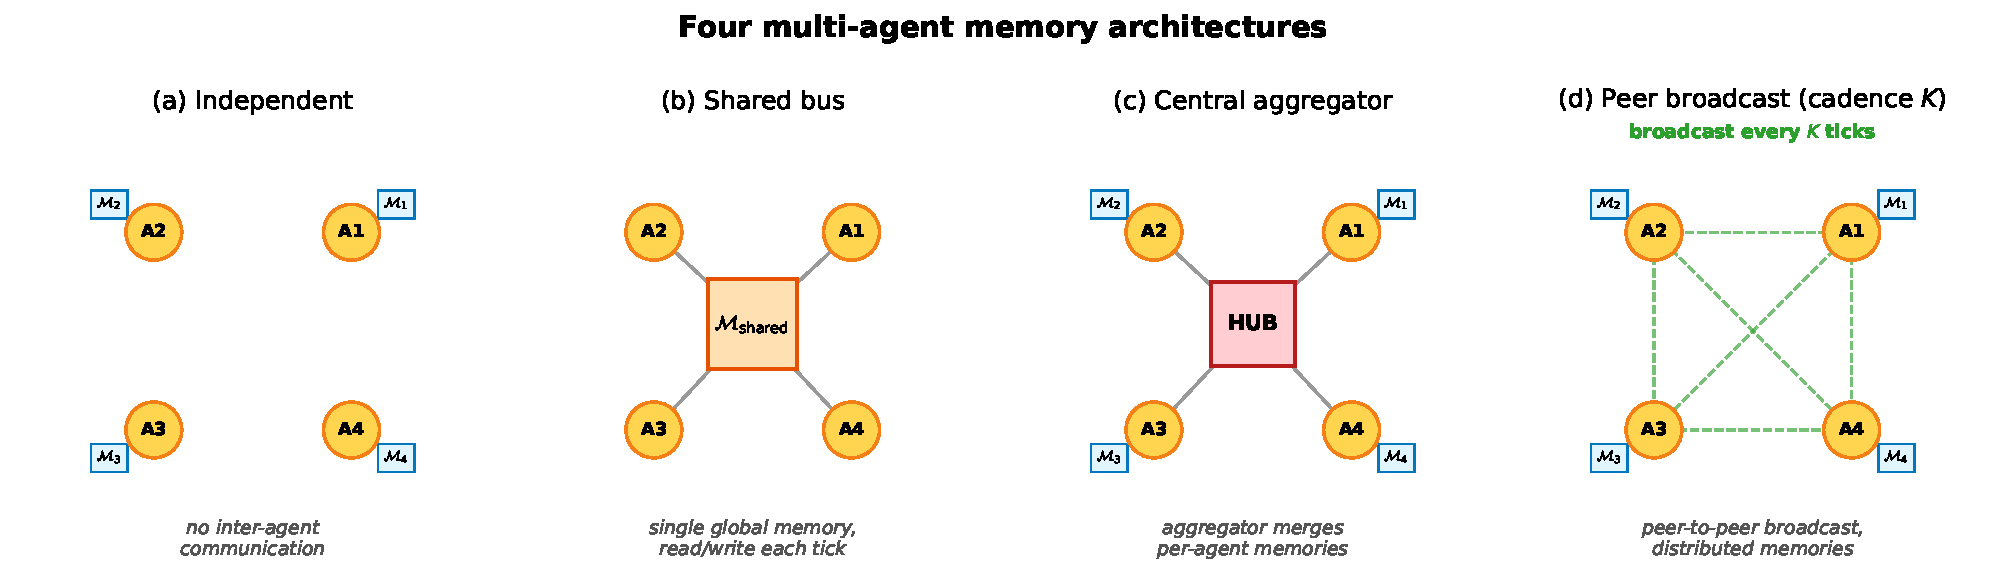
\includegraphics[width=\linewidth]{figures/fig_architectures.pdf}
  \caption{Четыре многоагентные архитектуры памяти. \textbf{(a)} Независимая: приватная память на агента, без обмена. \textbf{(b)} Общая шина: одна глобальная память, каждый агент читает/пишет каждый тик. \textbf{(c)} Центральный агрегатор: памяти агентов плюс хаб, сливающий их в консенсусный отчет. \textbf{(d)} Одноранговая рассылка: памяти агентов с попарным обменом снимками каждые $K$ тиков (ось каденции эмпирического утверждения~1).}
  \label{fig:architectures}
\end{figure}

\begin{description}[leftmargin=10pt,topsep=2pt,itemsep=2pt]
\item[Независимая.] Каждый агент поддерживает приватное хранилище событий и граф понятий. Механизм межагентной коммуникации отсутствует. Базовый метод нижней границы.
\item[Общая шина.] Все агенты публикуют наблюдения в единую шину событий \emph{коллективной памяти}. Один общий граф понятий перестраивается из объединения событий. Максимально централизованная.
\item[Центральный агрегатор (ConsensusLayer).] У каждого агента свой приватный граф понятий; центральный слой забирает снимки и вычисляет слияние, взвешенное доверием, порождая единый \emph{консенсусный отчет}, потребляемый всеми агентами.
\item[Одноранговая рассылка (каденция $K$).] У каждого агента свой граф понятий и свое слитое представление. Каждые $K$ тиков каждый агент рассылает снимок в пассивную шину; каждый агент независимо сливает свой снимок с последним снимком, полученным от каждого пира. Разные агенты могут держать разные слитые представления; центрального отчета нет.
\end{description}

Первые три соответствуют трем режимам в литературе по многоагентной
коммуникации: отсутствие обмена, агрегация в стиле CTDE и
децентрализованная одноранговая коммуникация. Четвертая --- архитектура, к которой
непосредственно применимы определение~2 и эмпирическое утверждение~1,
поскольку каденция $K$ --- настраиваемый параметр, а не
фиксированный протокол. Механически $K$ --- это скорость, с которой приватные
памяти консолидируются в коллективное представление, поэтому она и является
структурной осью этого раздела.

\subsection{Многоагентная факторизация}
\label{sec:multi-theory}

Расширим факторизацию на популяцию из $N$ агентов, разделяющих
информацию через коммуникационный протокол $\mathcal{C}_K$,
параметризованный каденцией рассылки $K$. Каждый агент $i$ имеет свое
состояние памяти $\mathcal{M}_i$ и выпускает свой запрос $q_i$. Пусть
$\mathcal{M}_i^{(K)}$ обозначает проекцию памяти агента $i$ в
момент запроса, после поглощения всех сообщений пиров, полученных
при каденции $K$. Разделяются два канала связывания: (i) связывание памяти
$\mathcal{M}_{-i}^{(K)}$ --- последние снимки памяти пиров,
доступные агенту $i$; (ii) связывание занятости $\mathcal{O}_{-i}$ ---
множество целей, уже занятых другими агентами к моменту,
когда действует $i$.

\paragraph{Определение 2 (многоагентная оцениваемость стадий).}
Для каждого агента $i$
\[
P(C^\star_i \mid q_i, \mathcal{M}_i, \mathcal{C}_K)
=
P(Q^\star_i \mid q_i, \mathcal{M}_i)\;
P(R^\star_i \mid Q^\star_i, q_i, \mathcal{M}_i, \mathcal{M}_{-i}^{(K)})
\]
\[
\quad \cdot\;
P(M^\star_i \mid R^\star_i, q_i, \mathcal{M}_i, \mathcal{M}_{-i}^{(K)})\;
P(C^\star_i \mid M^\star_i, q_i, \mathcal{O}_{-i}).
\]
При многоагентном стадийно-марковском предположении
(приложение~\ref{app:estimators}) четыре фактора оцениваемы из
поагентных журналов траекторий, а эмпирически-частотные оценки
состоятельны.

\paragraph{Когда определение~2 может нарушаться.}
Одноагентное стадийно-марковское свойство поглощает историю траектории в
$(q, \mathcal{M})$. В многоагентной постановке аналогичное
поглощение требует, чтобы зависимость от прошлых решений пиров входила только
через $\mathcal{M}_{-i}^{(K)}$ на стадии M и через
$\mathcal{O}_{-i}$ на стадии C. Этот шаг нетривиален:
$\mathcal{O}_{-i}$ суммирует занятость целей в момент решения, но
теряет информацию о том, \emph{как} пиры туда пришли.
Факторизация, следовательно, есть проекция на наблюдаемые поагентные
трассы при таком суммировании. Возникают два конкретных режима отказа: (i)
боковые каналы межагентной коммуникации, не логируемые через
$\mathcal{C}_K$; (ii) координированные политики пиров, чье решение на
стадии C зависит от скрытого состояния пиров, не суммируемого
$\mathcal{O}_{-i}$.

\subsection{Смещение бутылочного горлышка}
\label{sec:shift}

\paragraph{Эмпирическое утверждение~1 (смещение бутылочного горлышка M$\leftrightarrow$C, уровень наклонов).}
Предположим дефицит ($N > T$ целей, см.\ \S\ref{sec:notation}) и
архитектуру одноранговой рассылки с каденцией $K \in \mathbb{N}$. Постулируются два
стилизованных предположения:
\textbf{(F)} свежесть памяти $\nu(\mathcal{M}_{-i}^{(K)})$
поточечно не убывает при уменьшении $K$, и вероятность того, что
планировщик агента $i$ зафиксируется на достижимой цели, не убывает по
$\nu$;
\textbf{(O)} вероятность того, что произвольная зафиксированная цель
уже находится в $\mathcal{O}_{-i}$, не возрастает при увеличении $K$.
Запишем $P(M^\star|R^\star;K)$ и $P(C^\star|M^\star;K)$ для
популяционных условных вероятностей (усредненных по агентам и
распределению сидов бенчмарка); $\hat{P}(\cdot)$ обозначает
соответствующую эмпирически-частотную оценку, вычисленную из журналов. При
(F) и (O)
\[
\frac{\partial\, P(M^\star|R^\star;K)}{\partial K^{-1}} > 0,
\qquad
\frac{\partial\, P(C^\star|M^\star;K)}{\partial K^{-1}} < 0.
\]
Оба условия на наклоны --- прямые эмпирические предсказания,
проверяемые на журналах через $\hat{P}$.

\paragraph{Чем это утверждение является и чем не является.}
Эмпирическое утверждение~1 --- это \emph{утверждение об условных частотах на уровне наклонов}: каждый из двух наклонов проверяем и подтвержден при $p<10^{-4}$ на развертке из 35{,}640 прогонов (\S\ref{sec:multi-agent-results}) и независимо на развертке переносимости из 100 прогонов на стандартном MiniGrid ($p<10^{-6}$, \S\ref{sec:limitations}). Это \emph{не} утверждение о том, что условное произведение $\Phi(K) := P(M^\star|R^\star;K)\!\cdot\! P(C^\star|M^\star;K)$ имеет внутренний максимум; на наших данных $\Phi$ монотонно по $K$ на $\{4,8,16,32,48,64\}$ и сходится к границе независимых агентов $\Phi(K\!\to\!\infty){=}0.605$. Внутренний оптимум, порождаемый компромиссом M$\leftrightarrow$C, относится к практически значимой метрике эффективности --- среднему времени до успеха ($K{=}8$ на основной развертке), а не к $\Phi$. Мы не делаем формальных утверждений о $\Phi$.

\paragraph{Хронология.}
Эмпирическое утверждение~1 постфактумно. Оно было сформулировано \emph{после} первоначальной развертки из 12{,}960 прогонов, проведенной под четырьмя гипотезами, безразличными к стадиям (приложение~\ref{app:diagnostics}); два условия на наклоны были затем подтверждены на полной развертке из 35{,}640 прогонов, на масштабировании $N\!=\!12$ (приложение~\ref{app:babyai}) и на обертке переносимости для MiniGrid (\S\ref{sec:limitations}). Мы говорим это явно: проверенные знаки наклонов --- предсказания на расширенных данных, а не предварительно
зарегистрированное предсказание. Полностью формальная версия оставлена для будущей работы.

\subsection{Протокол развертки}
\label{sec:multi-agent-protocol}

Четыре архитектуры оцениваются на кастомной многоагентной сетке ($12{\times}10$ клеток); каждый агент должен достичь клетки с тегом \texttt{water\_source}, выбирая действия через общий планировщик, управляемый памятью, так что различается только слой памяти. Развертка пересекает $N{\in}\{3,5,8\}$, $T{\le}N$, три раскладки (симметричная/асимметричная/случайная), три плотности опасностей, четыре архитектуры, восемь одноранговых каденций $K{\in}\{1,2,4,8,16,32,48,64\}$, 40 сидов --- 35{,}640 прогонов за $\approx 22$ мин на 8 ядрах. Логируются поагентные потиковые индикаторы Q/R/M/C (приложение~\ref{app:estimators}); события уровня эпизода со звездочкой --- дизъюнкция по тикам. Отдельный блок оракульных интервенций на случаях дефицита $(N,T){\in}\{(3,2),(5,3),(8,5)\}$ при пяти каденциях оценивает оракульное R (память возвращает истинные позиции воды) и оракульное M (планировщик фиксируется на ближайшей реальной воде).

\subsection{Результаты: стадийная декомпозиция и смещение бутылочного горлышка}
\label{sec:multi-agent-results}

Развертка из 35{,}640 прогонов отчитывается через четыре наблюдения,
структурированных зеркально к эмпирическому утверждению~1: (i) условная
декомпозиция выделяет стадии M и C как различающие
звенья; (ii) смещение бутылочного горлышка проявляется непосредственно как отрицательная
внутрикаденционная корреляция между $P(M^\star|R^\star)$ и
$P(C^\star|M^\star)$ с пиком при $K\!=\!4$ и затуханием до шума при
$K\!=\!64$; (iii) на среднем времени до успеха возникающий компромисс
порождает чистый внутренний оптимум при $K\!=\!8$; (iv) на
условном произведении $\Phi$ тот же компромисс порождает монотонный
тренд, а не внутренний пик --- сводная статистика, о которой мы не делаем формальных утверждений. Базовый метод с обученной коммуникацией и многоагентный
цикл оракульных интервенций закрывают подраздел.

\subsubsection{Условная декомпозиция показывает, где отказывает каждая архитектура.}
Рисунок~\ref{fig:conditional-rates} показывает поархитектурные условные частоты Q/R/M/C; полная численная детализация с бутстреп-ДИ --- в приложении~\ref{app:phi-detail}, таблица~\ref{tab:multi-agent-cond}. Условная частота извлечения $P(R^\star|Q^\star)$ насыщена; различающий сигнал живет на M и C. Общая шина, центральный агрегатор и быстрая одноранговая рассылка ($K\le4$) имеют высокое $P(M^\star|R^\star)$, но низкое $P(C^\star|M^\star)$; независимая и медленная одноранговая ($K\ge16$) показывают обратное --- компромисс M$\leftrightarrow$C, предсказанный эмпирическим утверждением~1.

\begin{figure}[t]
  \centering
  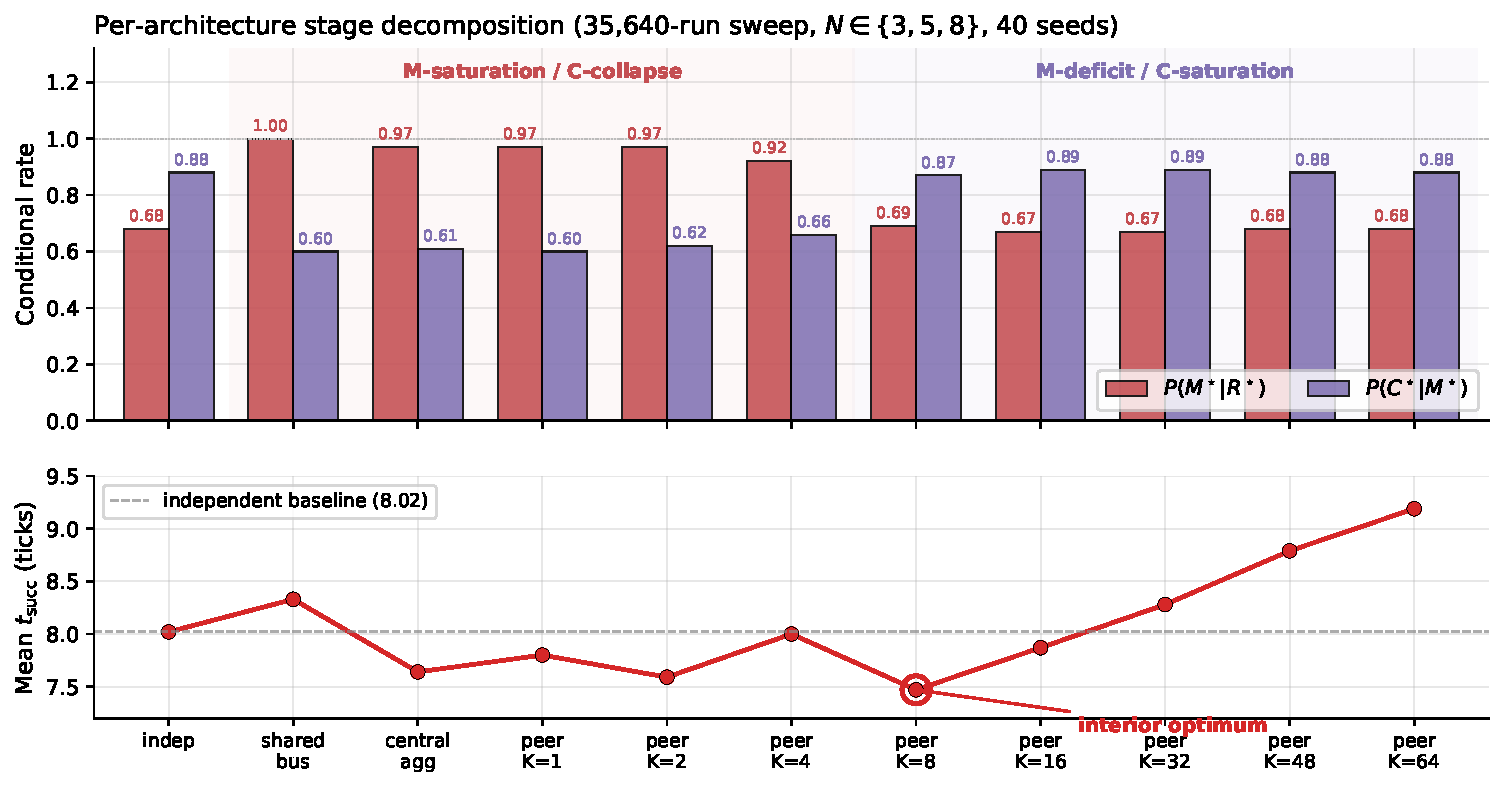
\includegraphics[width=\linewidth]{figures/fig_conditional_rates.pdf}
  \caption{Поархитектурные условные частоты (сверху) и среднее время до успеха (снизу) из развертки в 35{,}640 прогонов. Общая шина, центральный агрегатор и быстрая одноранговая рассылка ($K \le 4$) живут в режиме насыщения M / коллапса C; независимая и медленная одноранговая ($K \ge 16$) --- в режиме дефицита M / насыщения C. Среднее время до успеха имеет чистый внутренний минимум при $K{=}8$ ($7.47$ тика), ниже базового уровня независимых агентов ($8.02$).}
  \label{fig:conditional-rates}
\end{figure}


\subsubsection{Смещение бутылочного горлышка и внутренний оптимум эффективности.}
По всем одноранговым прогонам Спирмен для $P(M^\star|R^\star)$ против $K$ равен $-0.608$, а для $P(C^\star|M^\star)$ против $K$ равен $+0.420$ (оба $p<10^{-4}$), что соответствует условиям на наклоны из эмпирического утверждения~1. Более сильная эмпирическая сигнатура --- на уровне отдельных конфигураций: Пирсон для $P(M^\star|R^\star)$ против $P(C^\star|M^\star)$ \emph{внутри} фиксированного $K$ равен $-0.43, -0.54, -0.61, -0.19, -0.05, -0.04, -0.02, -0.02$ при $K{=}1,2,4,8,16,32,48,64$, с пиком при $K{=}4$ и затуханием до шума к $K{=}64$ (рисунок~\ref{fig:jensen-scatter}, приложение~\ref{app:phi-detail}). Конфигурации с высоким M систематически имеют низкое C: бутылочное горлышко мигрирует между двумя стадиями внутри одной и той же ячейки $(N,T,\text{раскладка},\text{опасность},\text{сид})$ при изменении $K$. На метрике эффективности среднее $t_{\mathrm{succ}}$ имеет U-образную форму с внутренним минимумом при $K{=}8$ (7.47 тика против 8.02 у независимого базового уровня; парные бутстреп-ДИ в приложении~\ref{app:phi-detail}). Масштабирование до $N{=}12$ \emph{обостряет} сигнатуру: пиковый Пирсон растет до $-0.70$ и
мигрирует наружу к $K\!=\!8$, что согласуется с тем, что более сильное связывание занятости
при большем $N$ откладывает переход режима стоимости
(приложение~\ref{app:babyai}, рисунок~\ref{fig:scale-n12}).

\paragraph{Чего мы не утверждаем о $\Phi$.} Условное произведение $\Phi = P(M^\star|R^\star)\!\cdot\!P(C^\star|M^\star)$ \emph{не} имеет внутреннего пика в проверенном диапазоне (оценка <<среднее произведений>> монотонно растет от $0.569$ при $K{=}4$ до $0.603$ при $K{=}64$, сходясь к границе независимых агентов $0.605$). Утверждение эмпирического утверждения~1 на уровне наклонов касается самих условных частот, а не $\Phi$; мы не делаем формальных утверждений о форме $\Phi(K)$. Детализация йенсеновского зазора и сравнение POM--MOP --- в приложении~\ref{app:phi-detail}.

\paragraph{Базовый метод с обученной коммуникацией: стадийные события структурно вырождены даже при конкурентоспособном успехе.}
Политика в стиле CommNet \citep{sukhbaatar2016commnet}, обученная PPO~\citep{schulman2017proximal} на том же сценарии ($N{=}3$, $T{=}2$), достигает $0.667$ успеха на отложенных сидах ($n{=}100$) --- на уровне символьной одноранговой архитектуры при $K{=}8$ ($0.65$). Несмотря на это, профиль Q/R/M/C остается структурно вырожденным: $Q^\star{=}1.00$ насыщено по построению; $R^\star{=}0.997$, $M^\star{=}0.997$ схлопнуты вместе ($P(M^\star|R^\star){=}1.00$). Это и есть проверенное структурное утверждение: вещественный коммуникационный вектор никогда не бывает информативно пустым (Q насыщается) и лишен явного интерфейса фиксации цели (R/M сливаются) независимо от бюджета обучения. Многоагентный аналог одноагентного анализа обученного BC (\S\ref{sec:single-results}). Полная архитектура, гиперпараметры PPO и параллельное сравнение REINFORCE и PPO --- в приложении~\ref{app:learned-baselines}.

\paragraph{Многоагентные оракульные интервенции замыкают цикл диагностика$\to$интервенция$\to$проверка.}
На случаях дефицита среднее $t_{\mathrm{succ}}$ при малой/промежуточной каденции ($K{\in}\{1,2,4\}$) падает с $\sim10$--$11$ в базовом режиме до $\sim7.1$ при оракульном R или оракульном M; при медленной каденции ($K{=}16$) базовый режим уже находится в пределах $\sim0.8$ от оракульного пола (таблица~\ref{tab:multi-agent-oracle} в приложении~\ref{app:multi-oracle}). Избыточное время, наведенное каденцией при малых/промежуточных $K$, атрибутируется переходу M$\leftrightarrow$C; при больших $K$ бутылочное горлышко переместилось в одиночную разведку.

Многоагентный блок тем самым вносит свою половину аргумента.
Каденция $K$ --- механически --- скорость, с которой приватные памяти
консолидируются в коллективное представление; данные показывают, что у этой скорости есть
нетривиальный внутренний оптимум ($K\!=\!8$ на $t_{\mathrm{succ}}$), что
ее канал стоимости --- связывание занятости, и что оба эффекта
видны постадийно на той же цепи Q/R/M/C, что и для одиночных
агентов. Консолидация --- не только одноагентный предел; в
коллективе это настраиваемая, измеримая ось проектирования.

\section{Минимальная коллективная семантическая память}
\label{sec:csm}
\label{sec:synthesis}

\subsection{От диагноза к пространству проектных решений}
Одноагентный диагноз (\S\ref{sec:refined-attribution}) локализовал самый трудный отказ не в механике извлечения, а в \emph{консолидации}: ранжирование кандидатов почти оптимально ($96.9\%$), но генерация голодает ($91\%$ пустых запросов). Многоагентный диагноз (\S\ref{sec:multi-agent-results}) показал, что тот же объект приобретает измеримую \emph{скорость}, когда консолидация разделяется. Четыре архитектуры из \S\ref{sec:archs} --- вырожденные углы более богатого пространства проектных решений: общая шина сливает все мгновенно (полная стоимость занятости), независимая не сливает никогда (полная стоимость устаревания), центральный агрегатор сливает через единственный доверенный хаб, одноранговая рассылка обнажает один параметр --- скорость $K$. Более богатая архитектура обнажает три явных правила: \textbf{слияние} (как объединяются свидетельства пиров об одном и том же месте), \textbf{доверие} (как взвешиваются конфликтующие или устаревшие свидетельства) и \textbf{устаревание} (как затухает консолидированная структура). Любую архитектуру, обнажающую все три правила, мы называем \emph{коллективной семантической памятью} (collective semantic memory, CSM) и инстанцируем здесь минимальную.

\subsection{Спецификация: минимальная CSM}
Минимальная CSM использует одноранговую рассылку при $K{=}8$ (лучшая фиксированная каденция на основной развертке) и накладывает три правила:
\begin{description}[leftmargin=14pt,itemsep=1pt,topsep=2pt]
\item[\textit{Слияние.}] Балл по месту: собственные свидетельства с весом 1, свидетельства пиров с весом $\mathrm{trust}_i \cdot e^{-\alpha \cdot \mathrm{age}}$, $\alpha = 0.05$. Порог $\tau = 0.30$ для включения в множество кандидатов.
\item[\textit{Доверие.}] Попировая EMA по согласованности успеха извлечения: пиры, чей последний разосланный снимок \emph{поддерживает} локально зафиксированную цель, набирают доверие; остальные затухают к $0.4$. Скорость обновления $\beta = 0.10$.
\item[\textit{Устаревание.}] Каждый разосланный снимок снабжен временной меткой; вес слияния на его свидетельствах затухает как $e^{-\alpha\cdot\mathrm{age}}$. Снимки старше $10K$ тиков вычищаются.
\end{description}

Код: \texttt{experiments/collective\_semantic\_memory/csm\_memory.py} (78 строк). CSM --- drop-in замена на том же логгере Q/R/M/C, что использован для четырех базовых архитектур.

\subsection{CSM строго доминирует над одноранговой рассылкой с фиксированной каденцией по доле успеха}
Мы сравниваем CSM с одноранговой рассылкой с фиксированной каденцией при $K \in \{1, 4, 8, 16, 64\}$ на полном многоагентном сценарии дефицита ($N \in \{3,5,8\}$ агентов, $T \in \{2,3,5\}$ целей, $N>T$; три раскладки, три плотности опасностей, 20 сидов): 540 прогонов на архитектуру, всего 3{,}240 за $\approx 5$ минут на одном ядре CPU. Таблица~\ref{tab:csm-results} приводит стадийно-условные частоты и сквозной успех.

\begin{table}[ht]
\caption{Минимальная коллективная семантическая память против одноранговой рассылки с фиксированной каденцией на сценарии дефицита (всего 3{,}240 прогонов, 20 сидов $\times$ 3 раскладки $\times$ 3 плотности опасностей $\times$ 3 ячейки дефицита $(N,T)$, $\approx 5$ мин настенного времени). \textbf{CSM строго доминирует над ВСЕМИ пятью одноранговыми архитектурами с фиксированной каденцией по сквозной доле успеха}: нижняя граница 95\%-го бутстреп-ДИ CSM (0.610) превышает верхнюю границу ДИ каждого однорангового $K$. В условной декомпозиции CSM занимает новую точку на плоскости (M$\,\times\,$C), недостижимую ни для одной фиксированной каденции.}
\label{tab:csm-results}
\centering
\small
\begin{tabular}{l c c c}
\toprule
Архитектура & $P(M^\star|R^\star)$ & $P(C^\star|M^\star)$ & Доля успеха (95\% ДИ) \\
\midrule
peer ($K{=}1$)  & 0.991 & 0.586 & 0.577 [0.572, 0.586] \\
peer ($K{=}4$)  & 0.955 & 0.623 & 0.581 [0.572, 0.590] \\
peer ($K{=}8$)  & 0.730 & 0.871 & 0.599 [0.591, 0.607] \\
peer ($K{=}16$) & 0.697 & 0.892 & 0.597 [0.589, 0.606] \\
peer ($K{=}64$) & 0.684 & 0.900 & 0.601 [0.594, 0.609] \\
\textbf{CSM (минимальная)} & \textbf{0.782} & \textbf{0.825} & \textbf{0.617 [0.610, 0.624]} \\
\bottomrule
\end{tabular}
\end{table}

Числа рассказывают согласованную историю. В условной декомпозиции ни одна одноранговая архитектура с фиксированной каденцией не достигает точки (0.78, 0.83) в пространстве $(P(M^\star|R^\star), P(C^\star|M^\star))$: быстрые рассылки ($K \le 4$) сидят в режиме насыщения M / коллапса C ($P(M^\star|R^\star) > 0.95$, $P(C^\star|M^\star) < 0.65$); медленные рассылки ($K \ge 16$) сидят в режиме дефицита M / насыщения C ($P(M^\star|R^\star) < 0.70$, $P(C^\star|M^\star) > 0.89$). CSM занимает третий режим, где и M, и C выше 0.78. Протокол измерения фреймворка обнаружил улучшение \emph{не} на каком-либо звене в изоляции, а в новой точке на плоскости M$\,\times\,$C, со следствием, что сквозная доля успеха строго выше (95\%-е бутстреп-ДИ не пересекаются со всеми одноранговыми $K$; $\Delta_{\mathrm{success}}\!\in\![+0.017, +0.040]$, все ДИ исключают ноль).

\subsection{Что CSM демонстрирует, а что нет}
Это \emph{минимальный} прототип: три простых правила поверх того же однорангового каркаса с $K=8$, без архитектурной новизны сверх явного контракта доверие/устаревание/слияние. Смысл его представления двоякий. Во-первых, заявленная в заголовке <<минимальная коллективная семантическая память>> предъявлена как инстанцированный артефакт, измеренный на той же шкале Q/R/M/C, что и четыре базовые архитектуры, а не как программное заявление. Во-вторых, показано, что протокол измерения фреймворка \emph{пригоден} для оценки новых архитектур: вклад CSM был бы невидим при отчетности только по успеху (абсолютный прирост $1.7\%$--$4.0\%$ выглядит маргинально), но отчетливо выделяется в условной декомпозиции, которую валидировала остальная часть статьи. Более богатые варианты CSM --- адаптивная каденция $K_t$, селективная консолидация недопредставленных семантических тегов, доверие, взвешенное намерениями, --- конкретные следующие шаги, перечисленные в приложении~\ref{app:open-problems}.

\section{Ограничения и будущая работа}
\label{sec:limitations}

\textbf{Переносимость между субстратами: условия на наклоны выполняются на MiniGrid.} Условия на наклоны из эмпирического утверждения~1 выполняются и на субстрате стандартного MiniGrid. Многоагентная обертка на основе FourRooms (построенная из \texttt{minigrid.core.grid.Grid} + примитивов Wall/Floor/Lava, идентичные операциональные определения $Q^\star,R^\star,M^\star,C^\star$; \texttt{experiments/minigrid\_multiagent\_wrapper/}) использовалась для развертки переносимости из 100 прогонов ($K{\in}\{1,4,8,16,64\}$, 20 сидов, $N{=}3$, $T{=}2$): Спирмен $P(M^\star|R^\star)$ против $K$ равен $-0.50$ ($p{=}1.5{\times}10^{-7}$), Спирмен $P(C^\star|M^\star)$ против $K$ равен $+0.50$ ($p{=}1.3{\times}10^{-7}$). Внутренний минимум $t_{\mathrm{succ}}$ не отделяется при таком минимальном размере развертки (5 каденций, 20 сидов, одна плотность опасностей); более плотная развертка --- естественный следующий шаг. Шов между двумя субстратами тем самым закрыт на уровне утверждения о наклонах.

\textbf{Эмпирическое утверждение~1 --- только уровень наклонов на условных частотах.} Два условия на наклоны выполняются ($p<10^{-4}$); мы не делаем формальных утверждений о форме условного произведения $\Phi$ (\S\ref{sec:shift}). Будущая формулировка непосредственно в терминах поверхности временной стоимости или вывод при порождающей модели (память с пуассоновским обновлением, занятость типа рождения--гибели) превратили бы эмпирическое утверждение в теорему.

\textbf{Оцениваемость при скрытом состоянии.} При нелогируемых внутриэпизодных переписываниях запросов или боковых каналах пиров определения~1 и~2 --- проекции на логируемые трассы, а не полная идентификация.

\textbf{Обученные базовые методы.} Базовый метод CommNet PPO достигает $0.667$ успеха на сценарии дефицита --- конкурентоспособно с символьной одноранговой архитектурой при $K{=}8$ ($0.65$) --- и подтверждает насыщение Q ($Q^\star{=}1.00$) и коллапс R/M ($P(M^\star|R^\star){=}1.00$) при конкурентоспособном успехе. Структурное предсказание теперь проверено, а не постулировано; абляция на архитектурах с явными символьными каналами фиксации цели оставлена для будущей работы.

\textbf{Масштаб.} Многоагентная развертка ограничена $N{=}12$ (приложение~\ref{app:babyai}; сигнатура обостряется, пиковый Пирсон $-0.70$ при $K{=}8$, внутренний минимум $t_{\mathrm{succ}}$ равен $4.77$). Более плотное масштабирование при $N{\ge}16$ и среды с непрерывным состоянием (например, VMAS~\citep{bettini2022vmas}) --- будущая работа.

\section{Более широкое влияние}

Статья предлагает диагностическую оценку для агентов на основе памяти в симулированной навигации. Ее позитивное влияние методологично: отказы на основе памяти становятся более измеримыми между архитектурами, а ось каденции распределенной многоагентной памяти --- настраиваемой по эмпирически обоснованному критерию. Потенциальные негативные влияния косвенны и возникли бы, если бы подобная диагностика использовалась для улучшения агентов в критичных к безопасности условиях (рои дронов, автономные транспортные средства, распределенные сенсорные сети) без адекватных мер защиты. Настоящая работа --- инфраструктура уровня бенчмарка, а не готовая к развертыванию система.

\section{Заключение}

Мы предложили Q/R/M/C --- четырехстадийную декомпозицию навигации на основе
памяти, факторы которой оцениваемы из стандартных журналов траекторий, ---
и использовали ее для проведения единого непрерывного аргумента: стадийная диагностика
локализует отказы, недоступные оценке только по успеху (одиночный агент);
когда память разделяется, каденция обмена становится измеримой
структурной осью с внутренним оптимумом (многоагентный случай); и оба
измерения локализуют связывающее ограничение в одном и том же механизме:
консолидации траекторных свидетельств в устойчивую, разделяемую
символьную структуру. Коллективная семантическая память --- разделяемая символьная
структура с явными правилами слияния, доверия и устаревания ---
поэтому не спекулятивное расширение, а исследовательская цель, на которую эти
результаты указывают, и представленный здесь фреймворк --- инструмент,
которым могут оцениваться кандидатные дизайны для нее.

\begin{ack}
Рукопись подготовлена в анонимизированной форме для рецензирования.
Отчитываемые эксперименты запускались из единого конвейера бенчмарков,
экспортирующего сводки по семействам задач, сравнения assist on/off,
диагностику методов, CSV многоагентных разверток и бутстреп-анализы из
одних и тех же эталонных артефактов бенчмарка.
\end{ack}

{\small
\begin{thebibliography}{9}

\bibitem[Andrychowicz et~al.(2017)]{andrychowicz2017hindsight}
M.~Andrychowicz, F.~Wolski, A.~Ray, J.~Schneider, R.~Fong, P.~Welinder, B.~McGrew, J.~Tobin, P.~Abbeel, and W.~Zaremba.
\newblock Hindsight experience replay.
\newblock In \emph{NeurIPS}, 2017.

\bibitem[B\v{e}lohl\'avek(1999)]{belohlavek1999fuzzy}
R.~B\v{e}lohl\'avek.
\newblock Fuzzy Galois connections.
\newblock \emph{Mathematical Logic Quarterly}, 45(4):497--504, 1999.

\bibitem[Bettini et~al.(2022)]{bettini2022vmas}
M.~Bettini, R.~Kortvelesy, J.~Blumenkamp, and A.~Prorok.
\newblock VMAS: A vectorized multi-agent simulator for collective robot learning.
\newblock In \emph{16th International Symposium on Distributed Autonomous Robotic Systems (DARS)}, 2022.
\newblock arXiv:2207.03530.

\bibitem[Boyd et~al.(2006)]{boyd2006gossip}
S.~Boyd, A.~Ghosh, B.~Prabhakar, and D.~Shah.
\newblock Randomized gossip algorithms.
\newblock \emph{IEEE Trans.\ Information Theory}, 52(6):2508--2530, 2006.

\bibitem[Chevalier-Boisvert et~al.(2018)]{chevalier2018babyai}
M.~Chevalier-Boisvert, D.~Bhoopchand, H.~Abdolmaleki, and A.~Mordatch.
\newblock BabyAI: A platform to study the sample efficiency of grounded language learning.
\newblock In \emph{ICLR}, 2019.

\bibitem[Chevalier-Boisvert et~al.(2023)]{MinigridMiniworld23}
M.~Chevalier-Boisvert, B.~Lahlou, S.~Willems, and P.~S. Castro.
\newblock MiniGrid and MiniWorld: Modular reinforcement learning environments.
\newblock \emph{arXiv:2306.13831}, 2023.

\bibitem[Dayan(1993)]{dayan1993improving}
P.~Dayan.
\newblock Improving generalization for temporal difference learning: The successor representation.
\newblock \emph{Neural Computation}, 5(4):613--624, 1993.

\bibitem[Deitke et~al.(2022)]{deitke2022procthor}
M.~Deitke, E.~V. Wijmans, D.~Schwenk, O.~Salvador, K.~M. Ehsani, et al.
\newblock ProcTHOR: Large-scale embodied AI using procedural generation.
\newblock In \emph{NeurIPS Datasets and Benchmarks}, 2022.

\bibitem[Efron(1979)]{efron1979bootstrap}
B.~Efron.
\newblock Bootstrap methods: Another look at the jackknife.
\newblock \emph{Annals of Statistics}, 7(1):1--26, 1979.

\bibitem[Foerster et~al.(2016)]{foerster2016learning}
J.~N. Foerster, Y.~M. Assael, N.~de~Freitas, and S.~Whiteson.
\newblock Learning to communicate with deep multi-agent reinforcement learning.
\newblock In \emph{NeurIPS}, 2016.

\bibitem[Foerster et~al.(2018)]{foerster2018ctde}
J.~N. Foerster, G.~Farquhar, T.~Afouras, N.~Nardelli, and S.~Whiteson.
\newblock Counterfactual multi-agent policy gradients.
\newblock In \emph{AAAI}, 2018.

\bibitem[Ganter and Wille(1999)]{ganter1999fca}
B.~Ganter and R.~Wille.
\newblock \emph{Formal Concept Analysis: Mathematical Foundations}.
\newblock Springer, 1999.

\bibitem[Ghosh et~al.(2021)]{ghosh2021learning}
D.~Ghosh, A.~Gupta, A.~Reddy, J.~Fu, S.~Levine, and C.~Finn.
\newblock Learning to reach goals via iterated supervised learning.
\newblock In \emph{ICLR}, 2021.

\bibitem[Gigerenzer and Goldstein(1996)]{gigerenzer1996reasoning}
G.~Gigerenzer and D.~G. Goldstein.
\newblock Reasoning the fast and frugal way: Models of bounded rationality.
\newblock \emph{Psychological Review}, 103(4):650--669, 1996.

\bibitem[Gupta et~al.(2017)]{gupta2017cognitive}
S.~Gupta, J.~Davidson, S.~Levine, R.~Sukthankar, and J.~Malik.
\newblock Cognitive mapping and planning for visual navigation.
\newblock In \emph{CVPR}, 2017.

\bibitem[Holm(1979)]{holm1979simple}
S.~Holm.
\newblock A simple sequentially rejective multiple test procedure.
\newblock \emph{Scandinavian Journal of Statistics}, 6(2):65--70, 1979.

\bibitem[Kolve et~al.(2017)]{kolve2017ai2thor}
E.~Kolve, R.~Mottaghi, D.~Gordon, Y.~Zhu, A.~Gupta, A.~Farhadi, and D.~Fox.
\newblock AI2-THOR: An interactive 3D environment for visual AI.
\newblock \emph{arXiv:1712.05474}, 2017.

\bibitem[Kuipers(2000)]{kuipers2000spatial}
B.~Kuipers.
\newblock The spatial semantic hierarchy.
\newblock \emph{Artificial Intelligence}, 119(1--2):191--233, 2000.

\bibitem[Lieder and Griffiths(2020)]{lieder2020resource}
F.~Lieder and T.~L. Griffiths.
\newblock Resource-rational analysis: Understanding human cognition as the optimal use of limited computational resources.
\newblock \emph{Behavioral and Brain Sciences}, 43:e1, 2020.

\bibitem[Lowe et~al.(2017)]{lowe2017maddpg}
R.~Lowe, Y.~Wu, A.~Tamar, J.~Harb, P.~Abbeel, and I.~Mordatch.
\newblock Multi-agent actor-critic for mixed cooperative-competitive environments.
\newblock In \emph{NeurIPS}, 2017.

\bibitem[Mac~Lane(1998)]{maclane1998categories}
S.~Mac~Lane.
\newblock \emph{Categories for the Working Mathematician}.
\newblock Springer, 2nd edition, 1998.

\bibitem[Momennejad et~al.(2017)]{momennejad2017successor}
I.~Momennejad, E.~M. Russek, J.~H. Cheong, M.~M. Botvinick, N.~Daw, and S.~J. Gershman.
\newblock The successor representation in human reinforcement learning.
\newblock \emph{Nature Human Behaviour}, 1:680--692, 2017.

\bibitem[O'Keefe and Nadel(1978)]{okeefe1978hippocampus}
J.~O'Keefe and L.~Nadel.
\newblock \emph{The Hippocampus as a Cognitive Map}.
\newblock Oxford University Press, 1978.

\bibitem[Packer et~al.(2023)]{packer2023memgpt}
C.~Packer, V.~Fang, S.~Patil, K.~Lin, S.~Wooders, and J.~Gonzalez.
\newblock MemGPT: Towards LLMs as operating systems.
\newblock \emph{arXiv:2310.08560}, 2023.

\bibitem[Savinov et~al.(2018)]{savinov2018semi}
N.~Savinov, A.~Dosovitskiy, and V.~Koltun.
\newblock Semi-parametric topological memory for navigation.
\newblock In \emph{ICLR}, 2018.

\bibitem[Savva et~al.(2019)]{savva2019habitat}
M.~Savva, A.~Kadian, O.~Maksymets, Y.~Zhao, E.~Wijmans, B.~Jain, J.~Straub, J.~Liu, V.~Koltun, J.~Malik, et al.
\newblock Habitat: A platform for embodied AI research.
\newblock In \emph{ICCV}, 2019.

\bibitem[Schulman et~al.(2016)]{schulman2016gae}
J.~Schulman, P.~Moritz, S.~Levine, M.~Jordan, and P.~Abbeel.
\newblock High-dimensional continuous control using generalized advantage estimation.
\newblock In \emph{ICLR}, 2016.
\newblock arXiv:1506.02438.

\bibitem[Schulman et~al.(2017)]{schulman2017proximal}
J.~Schulman, F.~Wolski, P.~Dhariwal, A.~Radford, and O.~Klimov.
\newblock Proximal policy optimization algorithms.
\newblock \emph{arXiv:1707.06347}, 2017.

\bibitem[Shinn et~al.(2023)]{shinn2023reflexion}
N.~Shinn, F.~Cassano, A.~Berman, and A.~G. Labash.
\newblock Reflexion: Language agents with verbal reinforcement learning.
\newblock In \emph{NeurIPS}, 2023.

\bibitem[Simon(1955)]{simon1955behavioral}
H.~A. Simon.
\newblock A behavioral model of rational choice.
\newblock \emph{Quarterly Journal of Economics}, 69(1):99--118, 1955.

\bibitem[Simon(1956)]{simon1956rational}
H.~A. Simon.
\newblock Rational choice and the structure of the environment.
\newblock \emph{Psychological Review}, 63(2):129--138, 1956.

\bibitem[Stachenfeld et~al.(2017)]{stachenfeld2017hippocampus}
K.~L. Stachenfeld, M.~M. Botvinick, and S.~J. Gershman.
\newblock The hippocampus as a predictive map.
\newblock \emph{Nature Neuroscience}, 20(11):1643--1653, 2017.

\bibitem[Sukhbaatar et~al.(2016)]{sukhbaatar2016commnet}
S.~Sukhbaatar, A.~Szlam, and R.~Fergus.
\newblock Learning multiagent communication with backpropagation.
\newblock In \emph{NeurIPS}, 2016.

\bibitem[Sutton et~al.(1999)]{sutton1999between}
R.~S. Sutton, D.~Precup, and S.~Singh.
\newblock Between MDPs and semi-MDPs: A framework for temporal abstraction in reinforcement learning.
\newblock \emph{Artificial Intelligence}, 112(1--2):181--211, 1999.

\bibitem[Tolman(1948)]{tolman1948cognitive}
E.~C. Tolman.
\newblock Cognitive maps in rats and men.
\newblock \emph{Psychological Review}, 55(4):189--208, 1948.

\bibitem[Wang et~al.(2023)]{wang2023voyager}
G.~Wang, Y.~Xie, Z.~Jiang, A.~Mandlekar, C.~Xie, A.~Yu, and P.~Liang.
\newblock Voyager: An open-ended embodied agent with large language models.
\newblock \emph{arXiv:2305.16291}, 2023.

\bibitem[Wilcoxon(1945)]{wilcoxon1945individual}
F.~Wilcoxon.
\newblock Individual comparisons by ranking methods.
\newblock \emph{Biometrics Bulletin}, 1(6):80--83, 1945.

\bibitem[Williams(1992)]{williams1992simple}
R.~J. Williams.
\newblock Simple statistical gradient-following algorithms for connectionist reinforcement learning.
\newblock \emph{Machine Learning}, 8(3--4):229--256, 1992.

\bibitem[Xiao et~al.(2007)]{xiao2007distributed}
L.~Xiao, S.~Boyd, and S.~Lall.
\newblock A scheme for robust distributed sensor fusion based on average consensus.
\newblock \emph{IPSN}, 2007.

\end{thebibliography}
}

\appendix

\section{Формальные доказательства}
\label{app:proofs}

\subsection{Аргумент для определения~1 (одноагентная оцениваемость)}

Для каждого эпизода $i \in \{1,\dots,n\}$ пусть $Q_i^\star, R_i^\star, M_i^\star, C_i^\star$ обозначают вложенные индикаторы уровня эпизода. По построению это измеримые функции журнала траектории времени исполнения, удовлетворяющие $C_i^\star \Rightarrow M_i^\star \Rightarrow R_i^\star \Rightarrow Q_i^\star$. Эмпирические оценки
\[
\hat p_Q = \tfrac{1}{n}\sum_i Q_i^\star,\quad
\hat p_{R|Q} = \tfrac{\sum_i R_i^\star}{\sum_i Q_i^\star},\quad
\hat p_{M|R} = \tfrac{\sum_i M_i^\star}{\sum_i R_i^\star},\quad
\hat p_{C|M} = \tfrac{\sum_i C_i^\star}{\sum_i M_i^\star}
\]
состоятельны по цепному правилу вместе с условным стадийно-марковским свойством, а эмпирическое произведение сходится к завершению семантического пути. \hfill$\square$

\subsection{Аргумент для определения~2 (многоагентная оцениваемость)}

Множества обусловливания расширяются за счет $\mathcal{M}_{-i}^{(K)}$ и $\mathcal{O}_{-i}$. При расширенном стадийно-марковском свойстве доказательство определения~1 переносится дословно, и каждая расширенная условная вероятность есть бернуллиевская вероятность на измеримом событии. Оговорки, сформулированные в \S\ref{sec:multi-theory} (<<Когда определение~2 может нарушаться>>), описывают две конкретные ситуации, в которых расширенное стадийно-марковское свойство нарушается. \hfill$\square$

\subsection{Аргумент для эмпирического утверждения~1 (формулировка на уровне наклонов)}

Эмпирическое утверждение~1 --- эмпирическое утверждение, а не теорема. Приведенный ниже аргумент --- качественное обоснование, мотивирующее два знака наклонов; проверяют же их данные. Мы сознательно не называем это доказательством.

\emph{Наклон (a), при (F).} При уменьшении $K$ величина $\nu(\mathcal{M}_{-i}^{(K)})$ поточечно не убывает. При условии успешного извлечения вероятность фиксации на достижимой цели не убывает по $\nu$. Следовательно, $\partial P(M^\star|R^\star;K) / \partial K^{-1} > 0$.

\emph{Наклон (b), при (O).} При уменьшении $K$ пиры получают обновленную память одновременно и сходятся к одной и той же ближайшей цели; маргинальная занятость $\Pr[\text{цель}\in\mathcal{O}_{-i}]$ растет. Следовательно, $\partial P(C^\star|M^\star;K) / \partial K^{-1} < 0$.

\emph{Замечание об условном произведении $\Phi$.} Эмпирическое утверждение~1 ничего не говорит о форме $\Phi(K) = P(M^\star|R^\star;K)\!\cdot\!P(C^\star|M^\star;K)$. При (F) и (O) наклон $\Phi$ по $K^{-1}$ есть сумма двух противоположных членов, и меняет ли он знак, зависит от количественных величин, не фиксируемых одними лишь (F) и (O). В наших данных $\Phi$ монотонно по $K$ на $\{4,8,16,32,48,64\}$ и сходится к границе независимых агентов $\Phi_\infty = 0.605$. Практически значимая поверхность эффективности --- среднее время до успеха --- действительно имеет внутренний минимум при $K=8$; см.\ \S\ref{sec:multi-agent-results}. \hfill$\square$

\subsection{Связь Галуа запрос--извлечение: формулировка, аргумент, область}
\label{app:galois}

\paragraph{Факт (стандартный).}
Пусть $G$ и $\Sigma$ --- множества, а $I \subseteq G \times \Sigma$ --- отношение. Для $B \subseteq \Sigma$ определим $\mathrm{ext}(B) = \{p \in G : \forall \tau \in B,\ (p,\tau) \in I\}$, а для $A \subseteq G$ определим $\mathrm{int}(A) = \{\tau \in \Sigma : \forall p \in A,\ (p,\tau) \in I\}$. Тогда для всех $A \subseteq G$, $B \subseteq \Sigma$:
\[
A \subseteq \mathrm{ext}(B) \iff B \subseteq \mathrm{int}(A);
\]
оба отображения антитонны, обе композиции $\mathrm{ext}\circ\mathrm{int}$ и $\mathrm{int}\circ\mathrm{ext}$ --- операторы замыкания, а замкнутые пары $(A, B)$ с $A = \mathrm{ext}(B)$ и $B = \mathrm{int}(A)$, упорядоченные по включению объемов, образуют полную решетку --- решетку понятий контекста $(G, \Sigma, I)$ \citep{ganter1999fca}.

\paragraph{Аргумент.}
$A \subseteq \mathrm{ext}(B)$ разворачивается в $\forall p \in A\ \forall \tau \in B:\ (p,\tau) \in I$ --- условие, симметричное по $A$ и $B$, что и есть в точности $B \subseteq \mathrm{int}(A)$. Антитонность и свойства замыкания следуют из стандартных однострочных аргументов \citep[гл.~1]{ganter1999fca}. Рассматривая булеаны как тонкие категории (одну с обращенным порядком), выписанная эквивалентность говорит ровно то, что $\mathrm{int}$ и $\mathrm{ext}$ образуют сопряженную пару; связь Галуа --- это сопряжение между посетами \citep[гл.~IV]{maclane1998categories}. \hfill$\square$

\paragraph{Инстанциация и область.}
В нашей памяти возьмем в качестве $G$ записи мест, в качестве $\Sigma$ --- алфавит тегов, а $I_\theta = \{(p,\tau) : \text{таблица тегов места назначает } \tau \text{ месту } p \text{ с уверенностью} \ge \theta\}$ (приложение~\ref{app:schemas}); намерение запроса --- это $B = q^{\mathrm{req}}$, а R-доступность --- это $\mathrm{ext}(B) \ne \emptyset$. Три сознательных ограничения области. (i) \emph{Градуированные баллы.} Развернутый балл извлечения градуирован (взвешенный лог-балл над обязательными, предпочтительными и штрафными тегами из приложения~\ref{app:schemas}), поэтому четкая связь выше формализует пороговый скелет кандидатства по обязательным тегам; градуированный аналог --- теория нечетких связей Галуа \citep{belohlavek1999fuzzy}, и здесь мы ее не используем. (ii) \emph{Немонотонные обновления.} Обновления Дирихле--мультиномиальные не являются буквально монотонными по $I_\theta$: противоположные свидетельства могут удалить инцидентность. На отчитываемых бенчмарках связывающий отказ --- это отсутствие свидетельств, а не противоречие (91\% пустых объемов, 96.9\% точности при непустых, \S\ref{sec:refined-attribution}), поэтому прочтение монотонного роста --- эмпирически релевантный режим, и мы помечаем исключение, а не отмахиваемся от него. (iii) \emph{Отсутствие структуры для M и C.} Материализация --- satisficing-функция выбора на непустых объемах, а завершение --- задача управления при занятости; ни одно из них не несет порядковой структуры, и мы не прикрепляем к ним категорных утверждений. Прочтение оправдывает свое место тем, что точно называет режим отказа (запрошенное намерение с пустым объемом лежит вне реализованной решетки понятий), дает консолидации точный объект (рост контекста, а значит и каждого объема) и структурно локализует ось каденции: связывание памяти $\mathcal{M}^{(K)}_{-i}$ сливает контексты пиров со скоростью $K^{-1}$, тогда как занятость $\mathcal{O}_{-i}$ экстраконтекстуальна --- в этом и состоит структурное содержание двух знаков наклонов эмпирического утверждения~1.

\section{Операциональные и вложенные стадийные оценки}
\label{app:estimators}

\paragraph{Операциональные диагностические частоты.}
Основной бенчмарк логирует познапросные и поэпизодные диагностические величины непосредственно из трасс времени исполнения (запрос сформирован, извлечение удовлетворено, цель материализована, завершение после извлечения). Это операциональные частоты, а не прямые мультипликативные факторы.

\paragraph{Вложенные стадийные оценки для факторизации.}
Для факторизации используются вложенные события уровня эпизода, полученные из первой отказавшей стадии, зафиксированной в таксономии времени исполнения: $Q^\star, R^\star, M^\star, C^\star$, вложенные по построению. Аудит согласованности в \S\ref{sec:validation} отчитывает $\hat P(Q^\star)$, $\hat P(R^\star|Q^\star)$, $\hat P(M^\star|R^\star)$, $\hat P(C^\star|M^\star)$, их произведение и его зазор до завершения семантического пути.

\subsection{Многоагентные операциональные определения}
\label{app:multi-agent-defs}

Для многоагентной развертки каждая метрика определяется на агента и на тик, затем агрегируется. Пусть $\mathrm{Targets}_i(t)$ --- множество кандидатов, возвращенное запросом к памяти агента $i$ на тике $t$, $\mathrm{Locked}_i(t)$ --- внутренняя для планировщика зафиксированная цель агента, а $\mathcal{W}$ --- истинное множество целей.

\textbf{Потиковые события.} $Q_i(t) = \mathbf{1}[\mathrm{Targets}_i(t) \ne \emptyset]$; $R_i(t) = \mathbf{1}[\exists w \in \mathcal{W}: \min_{c}\|c - w\| \le \epsilon]$ ($\epsilon = 0.6$); $M_i(t) = \mathbf{1}[\mathrm{Locked}_i(t) \ne \emptyset \land \min_w\|\mathrm{Locked}_i(t) - w\| \le \epsilon]$.

\textbf{События уровня эпизода со звездочкой.} $Q^\star_i = \bigvee_t Q_i(t)$; аналогично для $R^\star, M^\star$; $C^\star_i = \mathbf{1}[\text{агент } i \text{ достиг цели}]$.

\textbf{Агрегация.} Частоты по прогону усредняются по $N$ агентам; частоты по конфигурации усредняются по 40 сидам. Условные частоты $P(R^\star|Q^\star)$, $P(M^\star|R^\star)$, $P(C^\star|M^\star)$ вычисляются как отношения счетчиков уровня эпизода внутри каждой конфигурации до усреднения по конфигурациям.

\section{Схема памяти и задач}
\label{app:schemas}

\subsection{Полная таблица обозначений}
\label{app:notation}

Символы фиксированы на протяжении всей статьи.

\newcommand{\notentry}[1]{\par\smallskip\noindent\textbf{#1}\ \ }

\notentry{Стадии.}$Q$, $R$, $M$, $C$ --- четыре стадии: формирование запроса (\textbf{Q}uery), извлечение (\textbf{R}etrieval), материализация (\textbf{M}aterialization), завершение после извлечения (\textbf{C}ompletion). Они именуют как стадию, так и (в выражениях вида <<звено M>>) соответствующее ребро цепи.

\notentry{События.}$Q^\star, R^\star, M^\star, C^\star \in \{0, 1\}$ --- события уровня эпизода со звездочкой, фиксирующие успешность каждой стадии (приложение~\ref{app:estimators}). Вложены по построению: $Q^\star{=}1 \Leftarrow R^\star{=}1 \Leftarrow M^\star{=}1 \Leftarrow C^\star{=}1$.

\notentry{Вероятности.}$P(\cdot)$ --- популяционная вероятность (усредненная по распределению сидов и, в многоагентном случае, по агентам). $\hat{P}(\cdot)$ --- эмпирически-частотная оценка, вычисленная из журналов.

\notentry{Одиночный агент.}$q$ --- запрос; $\mathcal{M}$ --- состояние памяти; $Y$ --- сквозной успех задачи (может превышать $C^\star$).

\notentry{Многоагентный случай.}$N$ --- число агентов в популяции. $T$ --- число целей в среде (ограничение $T \le N$; <<дефицит>> означает $N > T$). $i$ --- индекс агента. $\mathcal{M}_i$ --- приватная память агента $i$. $q_i$ --- запрос агента $i$.

\notentry{Связывание.}$\mathcal{C}_K$ --- протокол одноранговой рассылки с каденцией $K \in \mathbb{N}$ (каждые $K$ тиков каждый агент рассылает снимок памяти, \S\ref{sec:archs}). $\mathcal{M}_{-i}^{(K)}$ --- последние снимки памяти пиров, доступные агенту $i$ при $\mathcal{C}_K$ (канал \emph{связывания памяти}). $\mathcal{O}_{-i}$ --- множество целей, уже занятых другими агентами к моменту действия $i$ (канал \emph{связывания занятости}).

\notentry{Переменные наклонов.}$\nu(\mathcal{M}_{-i}^{(K)})$ --- функционал свежести на памяти пиров; поточечно не убывает при уменьшении $K$ (предположение \textbf{(F)} эмпирического утверждения~1). Наклон занятости --- предположение \textbf{(O)}.

\notentry{Сводные статистики.}$\Phi(K) := P(M^\star|R^\star;K)\cdot P(C^\star|M^\star;K)$ --- условное произведение, цепная вероятность $P(M^\star \land C^\star \mid R^\star)$. POM (произведение средних) и MOP (среднее произведений) --- две оценки $\Phi$; они различаются на $\mathrm{Cov}(P(M^\star|R^\star), P(C^\star|M^\star))$, что и есть йенсеновский зазор (\S\ref{sec:multi-agent-results}). $t_{\mathrm{succ}}$ --- среднее время до успеха в тиках среды.
\par\smallskip

\subsection{Стек памяти и паттерны задач}

Стек памяти хранит символьные записи мест (пометные уверенности тегов, счетчики, посещаемость, свежесть, геометрия), записи переходов (статистики успеха, риска, стоимости с быстрыми/медленными оценками), эпизодические следы (намерение + состояние при каждом посещении) и записи понятий/отношений. На каждом шаге токенизатор испускает $(z_t, \tau_t, e_t)$ из $o_t$. Таблицы тегов мест используют Дирихле-мультиномиальное обновление; переходы --- экспоненциально сглаженные статистики; эпизодические записи прикрепляют активное намерение и состояние агента. Запрос планировщика обслуживается извлечением мест-кандидатов, чьи семантические профили соответствуют текущему намерению задачи и состоянию, через взвешенный лог-балл
$s(p \mid q_t, s_t) = \sum_{\tau \in q^{\mathrm{req}}} \log P(\tau|p)
+ \alpha \sum_{\tau \in q^{\mathrm{pref}}} \log P(\tau|p)
- \beta \sum_{\tau \in q^{\mathrm{pen}}} \log P(\tau|p)
+ \gamma\, u_{\mathrm{epi}}(p, s_t)$
над обязательными, предпочтительными и штрафными тегами. Четыре семейства задач определены семантическими паттернами мест: поиск воды (цель $\{$water$\}$), безопасный отдых ($\{$rest$\}$ с обусловливанием состоянием), возврат в целевую область ($\{$goal-region$\}$), восстановление после опасности ($\{$post-hazard-exit$\}$).

\subsection{Вспомогательные таблицы и рисунки для одиночного агента}
\label{app:single-results-table}

\begin{table*}[!ht]
  \caption{Лучший семантический результат по каждому семейству задач из финального 10-сидового бенчмарка, с 95\%-ми бутстреп-ДИ. Восстановление после опасности ограничено извлечением; целевая область остается ограниченной нисходящими стадиями.}
  \label{tab:main-results}
  \centering
  \scriptsize
  \setlength{\tabcolsep}{3.5pt}
  \begin{tabular}{p{1.5cm}p{1.7cm}c c c c c c c}
    \toprule
    Задача & Лучший метод & Assist & Успех (95\% ДИ) & Шаги & Запрос (оп.) & Извлеч.\ (оп.) & Матер.\ (оп.) & Пост (оп.) \\
    \midrule
    Вода & \method{water-cp} & on & 0.95 [0.88, 1.00] & 17.99 & 0.71 & 0.71 & 0.71 & 0.70 \\
    Отдых & \method{rest-s2} & on & 0.93 [0.85, 0.99] & 23.35 & 0.61 & 0.61 & 0.61 & 0.73 \\
    Целевая область & \method{goal-n1} & off & 0.54 [0.52, 0.56] & 49.34 & 0.00 & 0.00 & 0.00 & 0.00 \\
    Восст.\ после опасн. & \method{hazard-s7} & on & 0.40 [0.35, 0.45] & 10.18 & 0.11 & 0.11 & 0.11 & 0.16 \\
    \bottomrule
  \end{tabular}
\end{table*}

\begin{figure}[!ht]
  \centering
  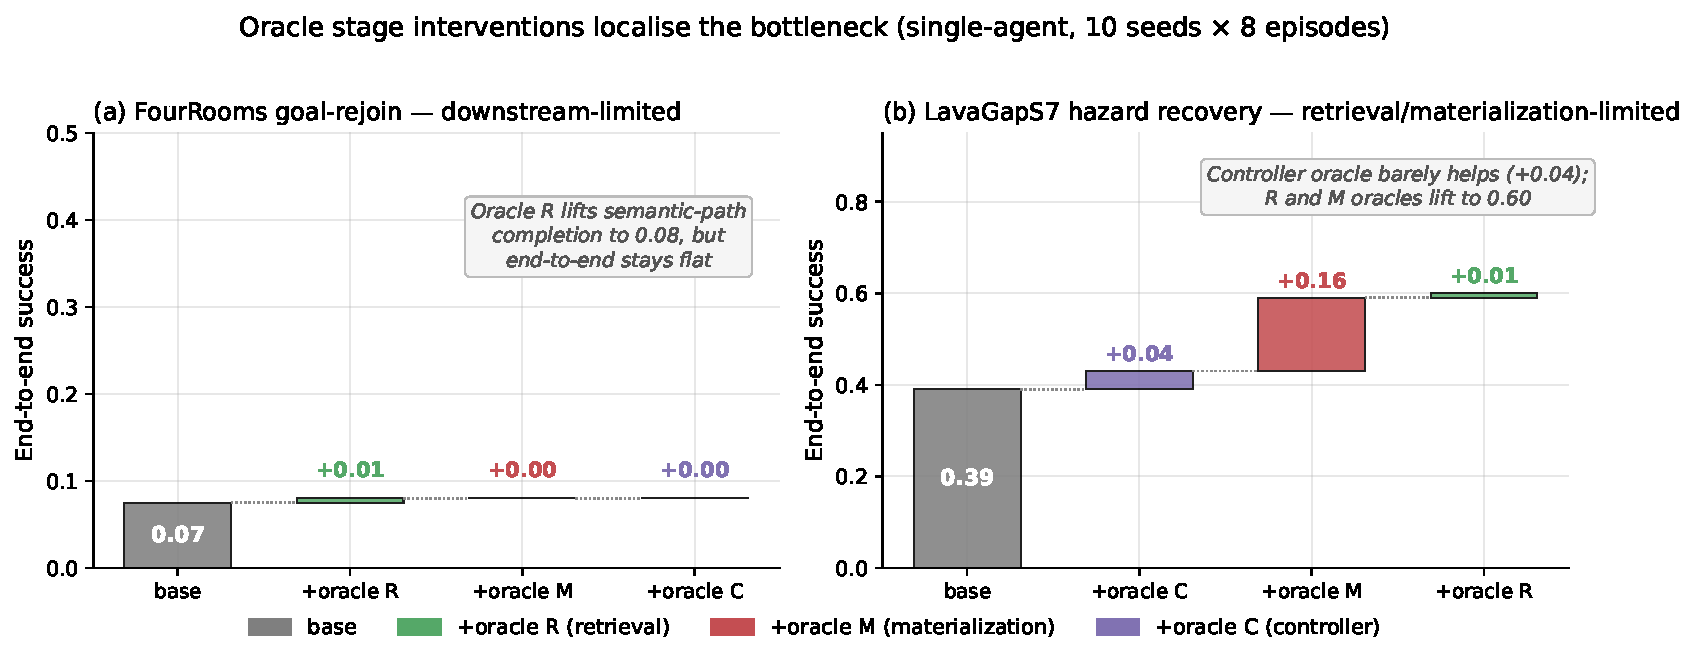
\includegraphics[width=\linewidth]{figures/fig_oracle_waterfall.pdf}
  \caption{Оракульные интервенции на стадиях для двух самых трудных одноагентных семейств задач (10 сидов $\times$ 8 эпизодов). \textbf{(a)} Возврат к цели в FourRooms: замена любой одной стадии оракулом оставляет сквозной успех на уровне $0.07$; бутылочное горлышко находится ниже стадий цепи. \textbf{(b)} Восстановление после опасности в LavaGapS7: оракульный контроллер добавляет лишь $+0.04$, но оракульная материализация добавляет $+0.16$, а оракульное извлечение --- еще $+0.01$, до $0.60$. Фреймворк локализует стадию бутылочного горлышка постадийно.}
  \label{fig:oracle-waterfall}
\end{figure}
\FloatBarrier

\section{Переносимость и масштабирование}
\label{app:babyai}

\subsection{Перенос на BabyAI (10 сидов, полный бенчмарк)}
\label{app:babyai-deeper}

10-сидовый бенчмарк переносимости на \texttt{BabyAI-GoToObjMaze-v0}~\citep{chevalier2018babyai} (8 эпизодов на сид, max-steps 200) измерил все четыре одноагентных метода основного бенчмарка (random, greedy, \texttt{babyai\_semantic\_node\_v1}, \texttt{babyai\_semantic\_plan\_v1}) с тем же логгером Q/R/M/C, примененным к трассам BabyAI. Числа в таблице~\ref{tab:babyai-deeper} подтверждают, что (a) события Q/R/M/C нетривиально испускаются на субстрате BabyAI, (b) два семантических варианта раскрывают стадийно-разделимую структуру там, где несемантические базовые методы имеют $Q^\star{=}R^\star{=}M^\star{=}0$ (семантические запросы не выпускаются), и (c) порядок стадийных частот совпадает с бенчмарком MiniGrid (таблица~\ref{tab:consistency}) в пределах бутстреп-ДИ. GoToObjMaze --- более трудный задачный субстрат, чем бенчмарк LavaGapS7/FourRooms основного текста --- сквозной успех ограничен 0.15 у всех методов, --- что делает стадийную декомпозицию особенно информативной: семантический стек не выигрывает по успеху, но является единственным семейством методов, порождающим измеримые постадийные события.

\begin{table}[h]
\centering
\caption{Бенчмарк переносимости на BabyAI: 10 сидов $\times$ 8 эпизодов на \texttt{BabyAI-GoToObjMaze-v0}, max-steps 200. Семантические варианты стека успешны с той же сквозной частотой, что и жадный базовый метод (0.15), но являются единственными методами, порождающими ненулевые события Q/R/M/C --- протокол фреймворка переносится на субстрат BabyAI без модификаций. Операциональные частоты Q/R/M/C здесь оцениваются на одном и том же знаменателе (число точек принятия решений), поэтому $Q{=}R{=}M$ для обоих семантических вариантов: GoToObjMaze испускает один тип семантической цели на эпизод.}
\label{tab:babyai-deeper}
\small
\begin{tabular}{l c c c c c c}
\toprule
Метод & Успех & Шаги & $Q$ (оп.) & $R$ (оп.) & $M$ (оп.) & Пост (оп.) \\
\midrule
random         & 0.125 $\pm$ 0.06 & 182.7 & 0.000 & 0.000 & 0.000 & 0.000 \\
greedy         & 0.150 $\pm$ 0.05 & 171.3 & 0.000 & 0.000 & 0.000 & 0.000 \\
semantic node  & 0.150 $\pm$ 0.05 & 171.3 & 0.032 & 0.032 & 0.032 & 0.025 \\
semantic plan  & 0.150 $\pm$ 0.05 & 171.3 & 0.032 & 0.032 & 0.032 & 0.025 \\
\bottomrule
\end{tabular}
\end{table}

\textbf{Вывод.} На второй субстрат переносится протокол измерения фреймворка --- а не его задачно-специфичные результаты. Сквозной успех на BabyAI определяется значительно более низким потолком успеха уровня эпизода в GoToObjMaze, а не стадийной структурой; и наоборот, стадийная структура, раскрываемая семантическим стеком, идентична по форме той, что тот же стек раскрывает на MiniGrid. Это ровно то свойство независимости от субстрата, которое методология и должна обеспечивать. Сырые данные: \texttt{tmp/babyai\_deeper\_10seed/}.

\subsection{Многоагентное масштабирование при $N=12$}
\label{app:scale-N12}

Чтобы проверить, что многоагентные результаты \S\ref{sec:multi-agent-results} --- не артефакт диапазона $N\!\le\!8$, была проведена дополнительная развертка из 8{,}640 прогонов при $N\!=\!12$, $T \in \{6, 8, 10\}$, тех же трех раскладках, трех плотностях опасностей, восьми одноранговых каденциях и 40 сидах. Настенное время $\approx 12$ минут на 8 ядрах. Сигнатура условных частот из \S\ref{sec:multi-agent-results} сохраняется и усиливается (таблица~\ref{tab:scale-n12}).

\begin{figure}[h]
\centering
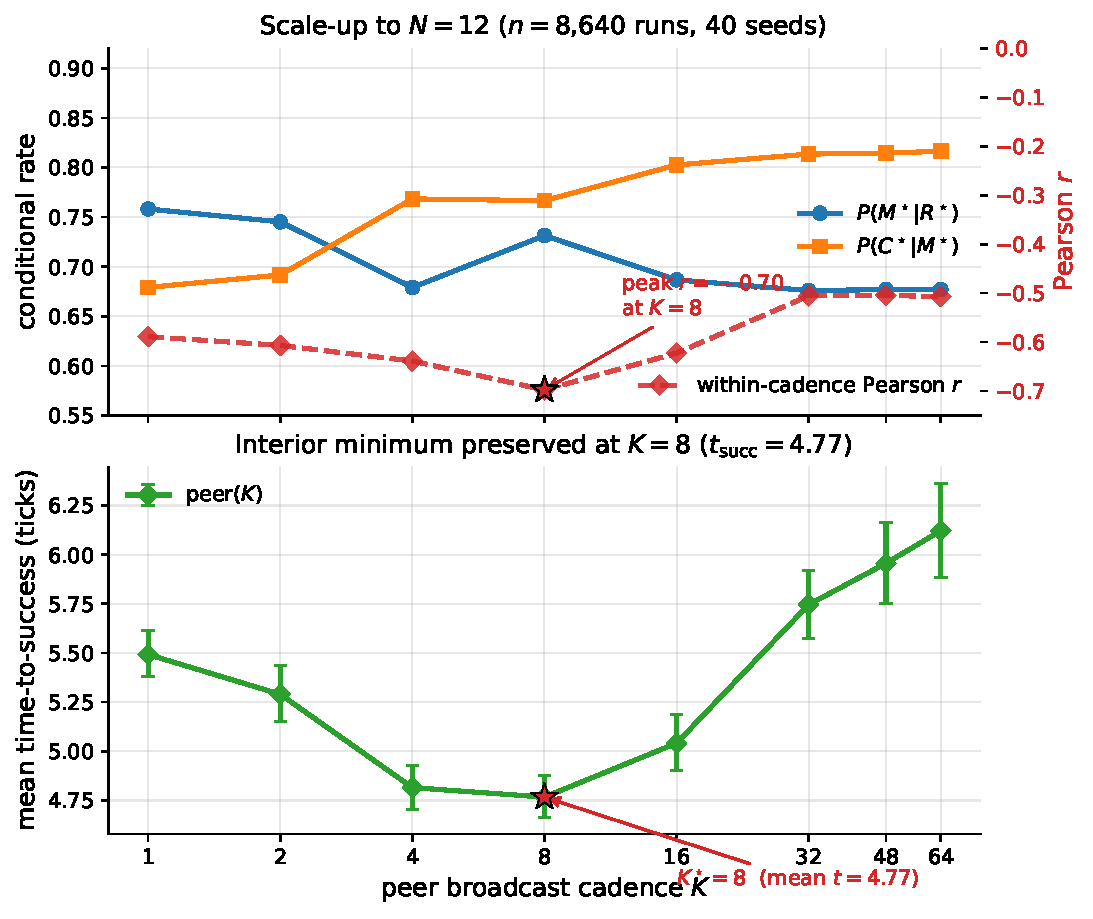
\includegraphics[width=0.92\linewidth]{figures/fig_scale_n12.pdf}
\caption{Сигнатура бутылочного горлышка при масштабировании до $N\!=\!12$ ($n\!=\!8{,}640$ прогонов, 40 сидов). Сверху: обе условные частоты меняются монотонно по $K$, как предсказано; внутрикаденционная корреляция Пирсона (красный пунктир, правая ось) достигает пика $-0.70$ при $K\!=\!8$. Снизу: среднее время до успеха сохраняет внутренний минимум при $K\!=\!8$ ($4.77$ тика). Пик смещения бутылочного горлышка мигрирует наружу от $K\!=\!4$ при $N\!\le\!8$ к $K\!=\!8$ при $N\!=\!12$, что согласуется с тем, что более сильное связывание занятости при большем числе агентов откладывает переход режима стоимости.}
\label{fig:scale-n12}
\end{figure}

\begin{table}[h]
\caption{Численная детализация развертки масштабирования $N\!=\!12$ (одноранговая архитектура). Условия на наклоны выполняются: Спирмен $P(M^\star|R^\star)$ с $K$ равен $-0.141$ ($p<10^{-39}$), а $P(C^\star|M^\star)$ с $K$ равен $+0.304$ ($p<10^{-184}$).}
\label{tab:scale-n12}
\centering
\small
\begin{tabular}{c c c c c c}
\toprule
$K$ & $P(M^\star|R^\star)$ & $P(C^\star|M^\star)$ & MOP & среднее $t_{\mathrm{succ}}$ & корр. \\
\midrule
1  & 0.758 & 0.679 & 0.475 & 5.49 & $-0.59$ \\
2  & 0.745 & 0.692 & 0.474 & 5.29 & $-0.61$ \\
4  & 0.679 & 0.768 & 0.482 & 4.82 & $-0.64$ \\
8  & 0.731 & 0.767 & 0.539 & \textbf{4.77} & $\mathbf{-0.70}$ \\
16 & 0.687 & 0.803 & 0.538 & 5.04 & $-0.62$ \\
32 & 0.676 & 0.814 & 0.538 & 5.75 & $-0.51$ \\
48 & 0.677 & 0.814 & 0.539 & 5.96 & $-0.51$ \\
64 & 0.677 & 0.816 & 0.541 & 6.12 & $-0.51$ \\
\bottomrule
\end{tabular}
\end{table}

\section{Расширенная диагностика}
\label{app:diagnostics}

\subsection{Детализация условного произведения и йенсеновский зазор}
\label{app:phi-detail}

\begin{table*}[h]
\caption{Поархитектурные условные частоты Q/R/M/C из развертки в 35{,}640 прогонов (40 сидов). $P(R^\star|Q^\star)$ насыщена. POM = произведение средних; MOP = среднее произведений (корректное поконфигурационное ожидаемое произведение). Две сводки систематически расходятся при малых/промежуточных $K$, потому что внутрикаденционная корреляция между $P(M^\star|R^\star)$ и $P(C^\star|M^\star)$ там сильно отрицательна (предпоследний столбец) --- сигнатура смещения бутылочного горлышка. \textbf{Жирным}: лучший MOP среди одноранговых каденций. Среднее $t_{\mathrm{succ}}$ (последний столбец) --- практически значимая мера эффективности; ее внутренний минимум при $K=8$ --- результат предсказанной формы, выдержавший данные.}
\label{tab:multi-agent-cond}
\centering
\scriptsize
\setlength{\tabcolsep}{3.5pt}
\begin{tabular}{l c c c c c c c}
\toprule
Архитектура & $P(R^\star|Q^\star)$ & $P(M^\star|R^\star)$ & $P(C^\star|M^\star)$ & POM & MOP (95\% ДИ) & корр. & среднее $t_{\mathrm{succ}}$ \\
\midrule
независимая          & 0.99 & 0.68 & 0.88 & 0.598 & 0.605 [0.597, 0.614] & $+0.00$ & 8.02 \\
общая шина           & 1.00 & 1.00 & 0.60 & 0.600 & 0.595 [0.586, 0.604] & $-0.10$ & 8.33 \\
центральный агрегатор & 1.00 & 0.97 & 0.61 & 0.592 & 0.572 [0.564, 0.580] & $-0.48$ & 7.64 \\
peer ($K=1$)         & 1.00 & 0.97 & 0.60 & 0.585 & 0.573 [0.564, 0.581] & $-0.43$ & 7.80 \\
peer ($K=2$)         & 1.00 & 0.97 & 0.62 & 0.594 & 0.576 [0.568, 0.584] & $-0.54$ & 7.59 \\
peer ($K=4$)         & 1.00 & 0.92 & 0.66 & 0.599 & 0.569 [0.561, 0.577] & $-0.61$ & 8.00 \\
peer ($K=8$)         & 0.99 & 0.69 & 0.87 & 0.597 & 0.586 [0.578, 0.595] & $-0.19$ & \textbf{7.47} \\
peer ($K=16$)        & 0.99 & 0.67 & 0.89 & 0.592 & 0.590 [0.581, 0.598] & $-0.05$ & 7.87 \\
peer ($K=32$)        & 0.99 & 0.67 & 0.89 & 0.595 & 0.598 [0.589, 0.606] & $-0.04$ & 8.28 \\
peer ($K=48$)        & 0.99 & 0.68 & 0.88 & 0.598 & 0.602 [0.593, 0.611] & $-0.02$ & 8.79 \\
peer ($K=64$)        & 0.99 & 0.68 & 0.88 & 0.599 & \textbf{0.603} [0.594, 0.611] & $-0.02$ & 9.19 \\
\bottomrule
\end{tabular}
\end{table*}

Условное произведение $\Phi = P(M^\star|R^\star)\!\cdot\!P(C^\star|M^\star)$ в развертке из 35{,}640 прогонов монотонно возрастает по $K$ на $K\in\{4,8,16,32,48,64\}$ и сходится к границе независимых агентов $\Phi(K\!\to\!\infty)=0.605$. Парный бутстреп: $\Delta(K{=}32{-}K{=}16) = +0.008$ (ДИ $[+0.006, +0.010]$), $\Delta(K{=}48{-}K{=}16) = +0.011$, $\Delta(K{=}64{-}K{=}16) = +0.012$; независимая значимо выше каждого однорангового $K$, кроме $K\!=\!64$ (на грани).

Отрицательная внутрикаденционная ковариация, задокументированная в \S\ref{sec:multi-agent-results}, создает зазор неравенства Йенсена между $\Phi$ и маргинальным произведением средних: $E[X]\!\cdot\!E[Y] > E[X\!\cdot\!Y]$ при $\mathrm{Cov}(X,Y) < 0$. Среднее произведений отчитывается как первичная сводка, поскольку оно корректно поглощает ковариацию. Рисунок~\ref{fig:bottleneck-shift} показывает $K$-развертку обеих условных частот и среднего $t_{\mathrm{succ}}$; рисунок~\ref{fig:jensen-scatter} показывает поконфигурационный скаттер, который отрицательная ковариация суммирует.

\begin{figure}[t]
  \centering
  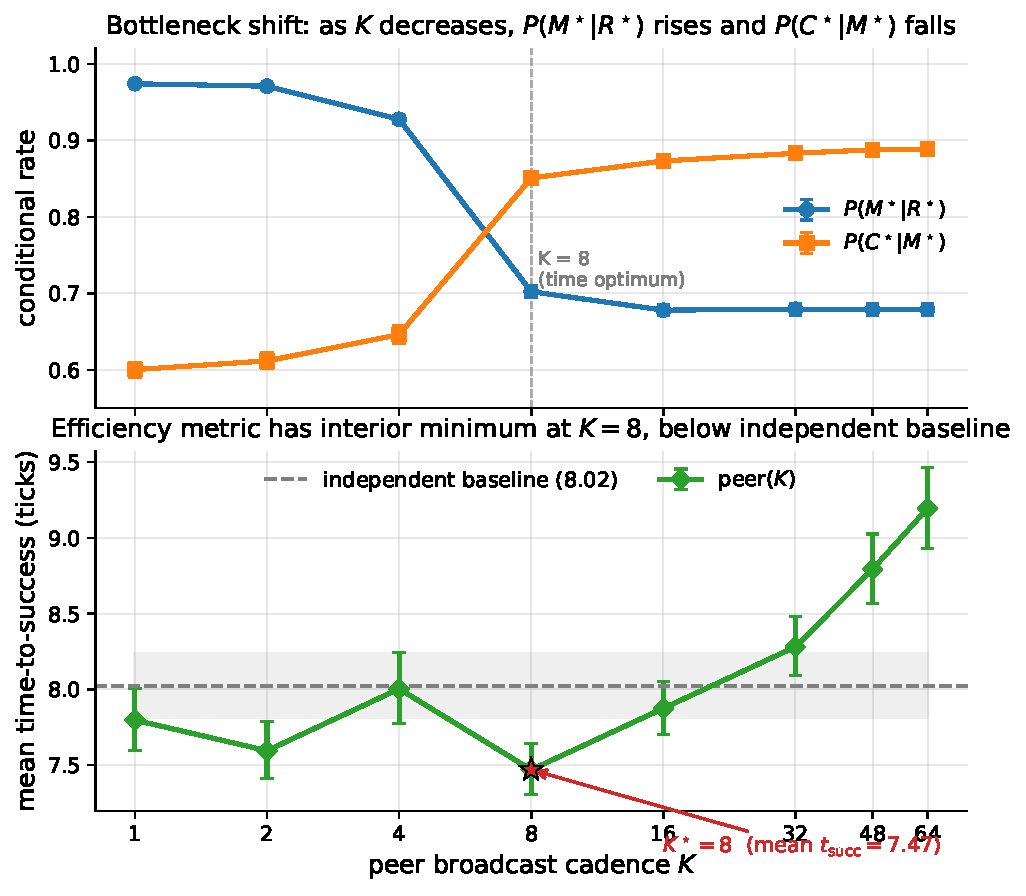
\includegraphics[width=0.85\linewidth]{figures/fig_bottleneck_shift.pdf}
  \caption{Смещение бутылочного горлышка по восьми одноранговым каденциям (развертка с 40 сидами). Сверху: $P(M^\star|R^\star)$ падает, а $P(C^\star|M^\star)$ растет монотонно по $K$ ($p<10^{-4}$, оба по Спирмену). Снизу: среднее время до успеха имеет внутренний минимум при $K=8$ ($7.47$ тика), ниже базового уровня независимых агентов ($8.02$, пунктир). Планки ошибок и закрашенная полоса --- 95\%-е бутстреп-ДИ.}
  \label{fig:bottleneck-shift}
\end{figure}

\begin{figure}[t]
  \centering
  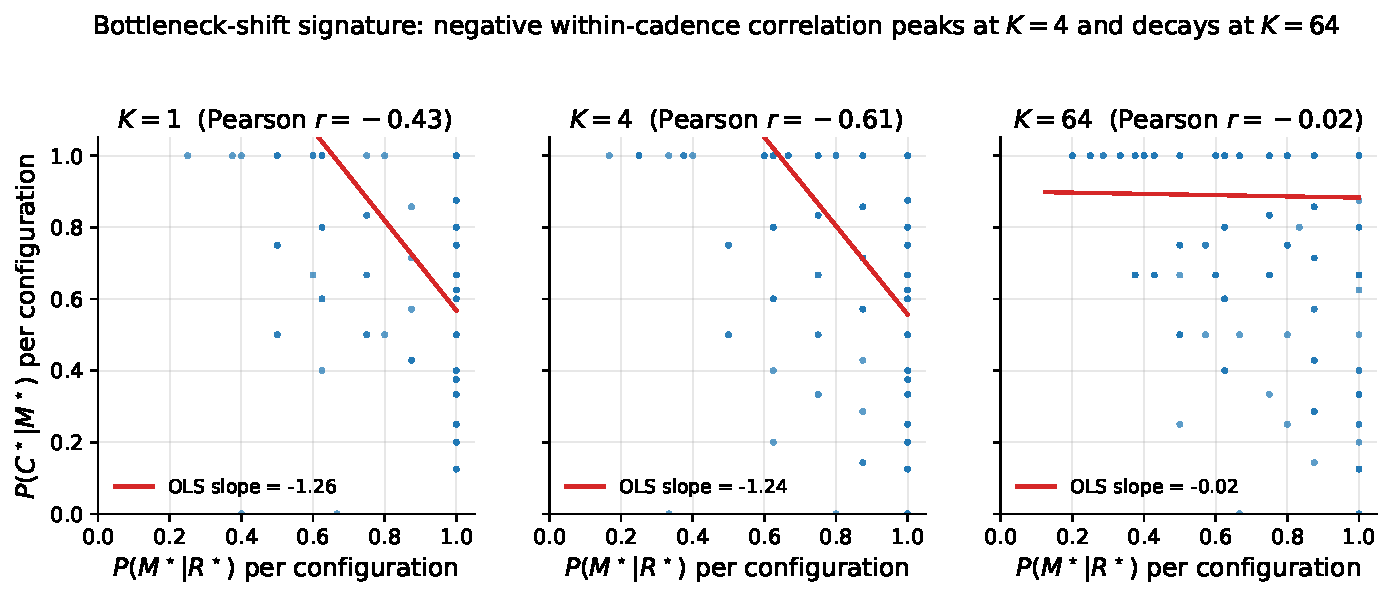
\includegraphics[width=0.95\linewidth]{figures/fig_jensen_scatter.pdf}
  \caption{Поконфигурационный скаттер $P(M^\star|R^\star)$ против $P(C^\star|M^\star)$ при трех каденциях. Сильная отрицательная корреляция при $K=4$ (Пирсон $-0.61$) --- сигнатура смещения бутылочного горлышка: те же конфигурации, что успешны на $M$, склонны отказывать на $C$, и наоборот. Корреляция затухает до шума к $K=64$.}
  \label{fig:jensen-scatter}
\end{figure}

\subsection{Открытые проблемы программы коллективной семантической памяти}
\label{app:open-problems}

Четыре конкретных вопроса напрямую следуют из измерений \S\ref{sec:multi-agent-results} и синтеза \S\ref{sec:synthesis}.
\textbf{(1) Адаптивная каденция.} Эмпирическое утверждение~1 предполагает фиксированное $K$; сигнатура смещения бутылочного горлышка подсказывает онлайн-контроллер $K_t$, который рассылает, когда (оцененный) выигрыш на стороне M превышает стоимость занятости на стороне C.
\textbf{(2) Селективная консолидация.} Обмен снимками сливает все подряд; правила слияния, приоритизирующие свидетельства о недопредставленных семантических тегах, атакуют голодание генерации кандидатов из \S\ref{sec:refined-attribution} напрямую.
\textbf{(3) Слияние, взвешенное доверием, при занятости.} Центральный агрегатор уже выполняет слияние, взвешенное доверием, но платит стоимость коллапса C; децентрализованные правила доверия, учитывающие \emph{намерения} пиров (а не только их свидетельства), могли бы расцепить свежесть и гонку за целями.
\textbf{(4) Общность субстратов.} Декомпозиция переносится между MiniGrid, BabyAI, кастомной сеткой и теперь многоагентной оберткой стандартного MiniGrid с идентичными операциональными определениями и проверенными знаками наклонов эмпирического утверждения~1 ($\S$~\ref{sec:limitations}). Среда с непрерывным состоянием (Habitat~\citep{savva2019habitat}, VMAS~\citep{bettini2022vmas}) --- оставшийся шаг переносимости.

\subsection{Расширенный обзор литературы}
\label{app:related-work-extended}

Классические взгляды на когнитивные карты мотивируют явные абстракции мест \citep{tolman1948cognitive,okeefe1978hippocampus,kuipers2000spatial}; современный воплощенный ИИ сочетает картирование и планирование \citep{gupta2017cognitive} или обнажает топологическую память (SPTM, \citealp{savinov2018semi}); целеобусловленный RL обусловливается явными целями или эмбеддингами \citep{andrychowicz2017hindsight,ghosh2021learning}, а работы о представлении преемника дают предсказательную структуру \citep{dayan1993improving,stachenfeld2017hippocampus,momennejad2017successor}. Наша постановка отличается тем, что цель --- это семантический паттерн, извлекаемый из памяти, а не координата. В многоагентном RL доминирует CTDE \citep{lowe2017maddpg,foerster2018ctde}, а обученная коммуникация добавляет пошаговую переменную обмена \citep{sukhbaatar2016commnet,foerster2016learning}; протоколы gossip и консенсуса \citep{boyd2006gossip,xiao2007distributed} --- ближайший сетевой аналог нашей оси каденции, поднятой здесь на уровень когнитивной архитектуры. Системы LLM-агентов опираются на явную память, но оцениваются сквозным образом \citep{wang2023voyager,shinn2023reflexion,packer2023memgpt}. Наш фреймворк ортогонален: вместо сквозного обучения коммуникационной политики он \emph{диагностирует}, где в цепи Q/R/M/C данная архитектура успешна или неуспешна, и дает проверяемое на журналах предсказание о каденции на уровне наклонов.

\subsection{Численная детализация многоагентных оракульных интервенций}
\label{app:multi-oracle}

\begin{table}[h]
\caption{Многоагентные оракульные интервенции на случаях дефицита при трех каденциях. Среднее время до успеха, усредненное по $(N,T)\in\{(3,2),(5,3),(8,5)\}$, двум раскладкам (асимметричная, случайная), 15 сидам.}
\label{tab:multi-agent-oracle}
\centering
\small
\begin{tabular}{c c c c c}
\toprule
$K$ & Базовый & Оракул R & Оракул M & Зазор до оракула \\
\midrule
1  & 10.33 & 7.22 & 7.08 & $-3.11$ \\
4  & 10.97 & 7.22 & 7.08 & $-3.75$ \\
16 &  7.98 & 7.22 & 7.08 & $-0.76$ \\
\bottomrule
\end{tabular}
\end{table}

\subsection{Безразличные к стадиям каденционные гипотезы и что меняет фреймворк}
\label{app:standalone-hypotheses}

Первая версия многоагентной каденционной развертки (12{,}960 прогонов при 20 сидах; поглощена разверткой из 35{,}640 прогонов в этой статье) изначально планировалась под четырьмя операциональными гипотезами, сформулированными \emph{до} эмпирического утверждения~1. Они сохранены здесь, потому что мотивировали итоговый фреймворк. Фреймворк был сформулирован после завершения развертки; не утверждается, что он априори предсказал числа развертки (см.\ <<Хронологию>> в \S\ref{sec:shift}).

\textbf{Исходные гипотезы (до фреймворка).}
\begin{description}[leftmargin=10pt,topsep=2pt,itemsep=1pt]
\item[H1.] Внутреннее $K^\star \in \{2,4,8\}$, минимизирующее среднее время до успеха, существует для большинства ячеек $(N, T, \text{раскладка})$.
\item[H2.] $K^\star$ монотонно растет с дефицитом $\rho = N/T$.
\item[H3.] При $\rho \le 1$ выполняется $K^\star = 1$.
\item[H4.] Одноранговые архитектуры рассылки Парето-доминируют централизованную агрегацию по (среднее время до успеха, доля успеха).
\end{description}

\textbf{Автономный результат на исходной развертке с 20 сидами.}
Практическое утверждение подтвердилось: одноранговая при эмпирически лучшем $K$ была быстрее централизованной в режиме дефицита ($p = 0.044$, Манн--Уитни). Из четырех структурных гипотез только H4 отчетливо подтвердилась на подмножестве случайных раскладок. H1 выполнялась в 7 из 18 ячеек; H2 имела незначимую отрицательную корреляцию; H3 подтвердилась в 4 из 9 допустимых ячеек. Расширенная развертка из 35{,}640 прогонов, используемая в остальной части статьи, дает совпадающие автономные числа в пределах бутстреп-неопределенности.

\textbf{Что меняет фреймворк.}
Гипотезы H1--H4 безразличны к стадиям: каждая связывает $K^\star$ с дефицитом $\rho$, не специфицируя механизм. Эмпирическое утверждение~1, сформулированное после развертки, связывает наклоны $P(M^\star|R^\star)$ и $P(C^\star|M^\star)$ с каденцией; условия на наклоны проверяемы на журналах. Данные верифицируют оба знака ($p<10^{-4}$). Мы не делаем формальных утверждений о форме условного произведения $\Phi$, по которому данные монотонны. Внутренний оптимум выполняется на метрике эффективности --- среднем времени до успеха.

\section{Анализ assist on/off}
\label{app:assist}

По всем четырем одноагентным семействам задач итоговый успех практически не меняется при assist on/off ($\Delta \le 0.10$). Единственный нетривиальный эффект --- на отдыхе, где ассисты улучшают завершение после извлечения на~$+0.05$, не меняя частот запроса/извлечения, что согласуется с действием ассистов на материализацию и исполнение после извлечения.

\section{Дообученный ретривер и базовый метод CommNet}
\label{app:learned-baselines}

\subsection{Дообученный MLP генерации кандидатов (\S\ref{sec:refined-attribution})}

\textbf{Извлечение датасета.} Из 10-сидового бенчмарка восстановления после опасности
(MiniGrid-LavaGapS7-v0, метод \texttt{milestone\_state\_conditioned\_hazard\_recovery\_v7})
извлекался 18-мерный вектор признаков для каждого шага каждого эпизода каждого сида --- 3 числовых скаляра состояния агента (energy, thirst, risk\_budget),
9 уверенностей семантических тегов, 6 one-hot намерений --- и бинарная метка: \emph{был
ли этот символьный узел когда-либо выбран кандидатом в течение прогона?} Итоги датасета:
814 примеров, 113 позитивных (13.9\%).

\textbf{Разбиение.} По сидам: train $\{2,3,4,5,6,7\}$ (505 примеров, 9.7\% позитивных),
val $\{8,9\}$ (170, 22.4\% позитивных), test $\{10,11\}$ (139, 18.7\% позитивных).

\textbf{Архитектура.} $18 \to 32 \to 32 \to 1$, активации ReLU, BCE с
$\text{pos\_weight}\!\approx\!9.3$ для дисбаланса классов, Adam $\text{lr}=2{\cdot}10^{-3}$
с $\text{weight\_decay}=10^{-4}$, батч 64, 200 эпох, лучший по val loss.

\textbf{Результаты.}

\begin{table}[h]
\centering
\small
\begin{tabular}{l c c c}
\toprule
Метрика & Train & Val & Test \\
\midrule
Точность                          & 0.584 & 0.553 & 0.590 \\
Точность мажоритарного класса     & 0.903 & 0.776 & 0.813 \\
Precision @ recall $=0.70$        & 0.171 & 0.278 & 0.275 \\
\bottomrule
\end{tabular}
\end{table}

\begin{figure}[h]
\centering
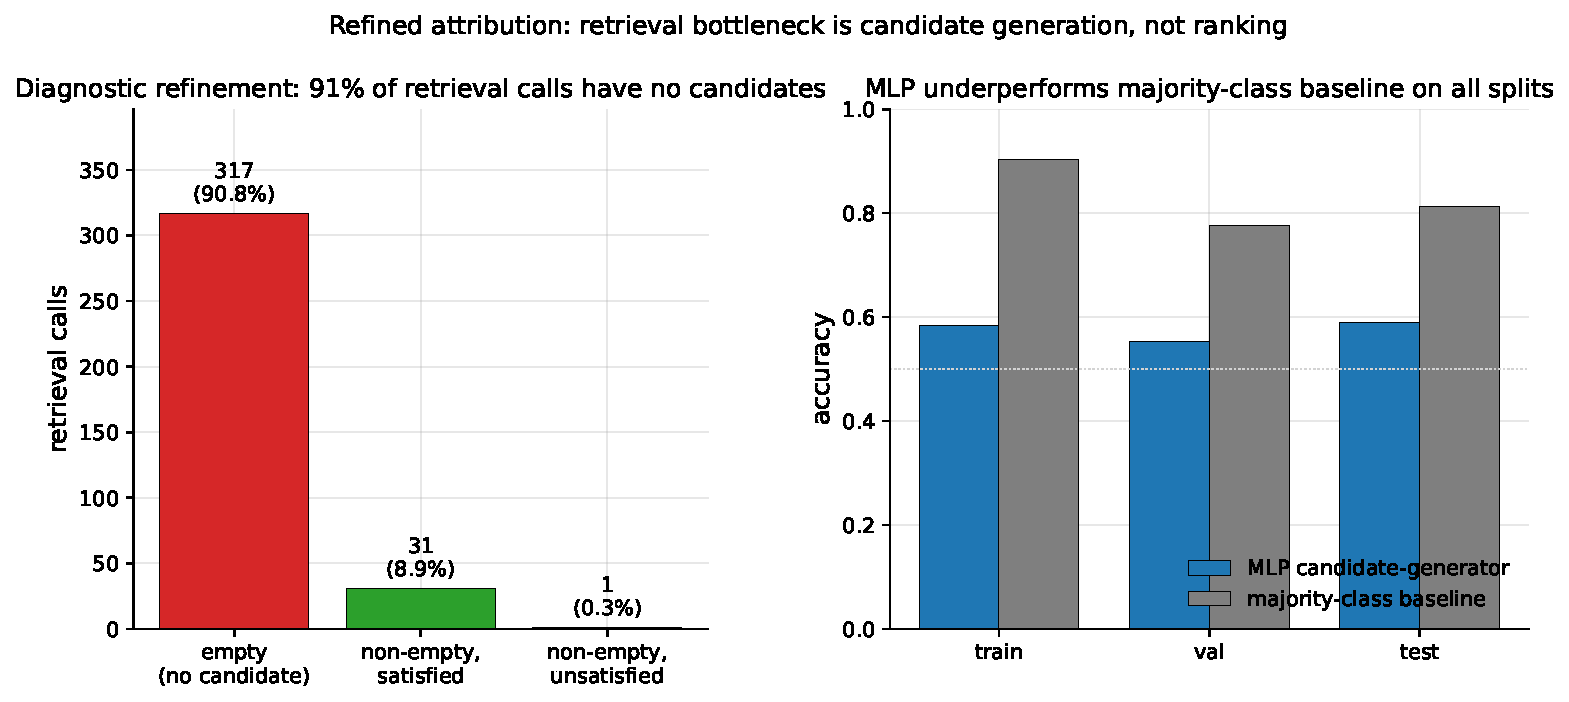
\includegraphics[width=0.95\linewidth]{figures/fig_refined_attribution.pdf}
\caption{Диагностика уточненной атрибуции. \emph{Слева:} 349 вызовов извлечения, агрегированных по 10 сидам; 317 (90.8\%) вернули пустые множества кандидатов, 31 (8.9\%) вернул хотя бы одного удовлетворяющего кандидата, лишь 1 (0.3\%) вернул кандидатов, которые были ранжированы, но не удовлетворяли. Бутылочное горлышко --- генерация кандидатов, а не их ранжирование. \emph{Справа:} обученный MLP уступает мажоритарному базовому методу на всех трех сид-дизъюнктных разбиениях, подтверждая, что одних мгновенных признаков состояния недостаточно для предсказания пригодности кандидата.}
\label{fig:refined-attribution}
\end{figure}

MLP уступает мажоритарному классу по точности на всех разбиениях и
достигает лишь умеренной precision при фиксированном recall. Мгновенных признаков
состояния недостаточно для предсказания пригодности кандидата ниже по конвейеру. Это
негативная, но информативная находка, на которую ссылается \S\ref{sec:refined-attribution}:
атрибуция фреймворка <<ограничено извлечением>> уточняется до
<<ограничено накоплением памяти>>, а не <<ограничено ранжированием>>.

\subsection{Базовый метод обученной коммуникации в стиле CommNet (\S\ref{sec:multi-agent-results})}

\textbf{Архитектура политики.} Наблюдение агента --- 4-мерный one-hot направления
$+$ локальное окно типов клеток $5\!\times\!5\!\times\!5$ (125) $+$ 2-мерная нормированная
позиция $=$ 131. Энкодер с общими весами $131{\to}64{\to}64$ (ReLU), 16-мерная
проекция коммуникации, среднее по пирам (исключая себя), объединение $80{\to}64$ (ReLU),
голова актора $64\!\to\!4$ (TURN\_LEFT, TURN\_RIGHT, FORWARD, NOOP), голова критика
$64\!\to\!1$. Это архитектура обученной коммуникации в стиле CommNet~\citep{sukhbaatar2016commnet}.

\textbf{Обучение.} REINFORCE~\citep{williams1992simple} с бейзлайном-ценностью; loss $=\!-\,\mathrm{mean}(\log\pi(a)\cdot(R\!-\!V))\,+\,0.5\cdot\mathrm{MSE}(V,R)\,-\,0.01\cdot H[\pi]$; Adam $\text{lr}=3{\cdot}10^{-4}$, клиппинг градиента $1.0$. Шейпинг награды: $+1.0$ за первый успех на агента, $-0.01$ стоимость шага, $-0.1$ за контакт с опасностью. 2000 эпизодов с циклом по 200 сидам среды, настенное время $100$\,с на CPU. Отложенная оценка: 50 сидов среды 250--299.

\textbf{Кривая обучения.} Успех уровня эпизода (окно последних 100) остается в
$[0.13, 0.23]$ на протяжении обучения; монотонного улучшения после $\sim\!200$
эпизодов нет. Политика сходится к локальному оптимуму, где один из трех агентов
находит воду случайно.

\begin{figure}[h]
\centering
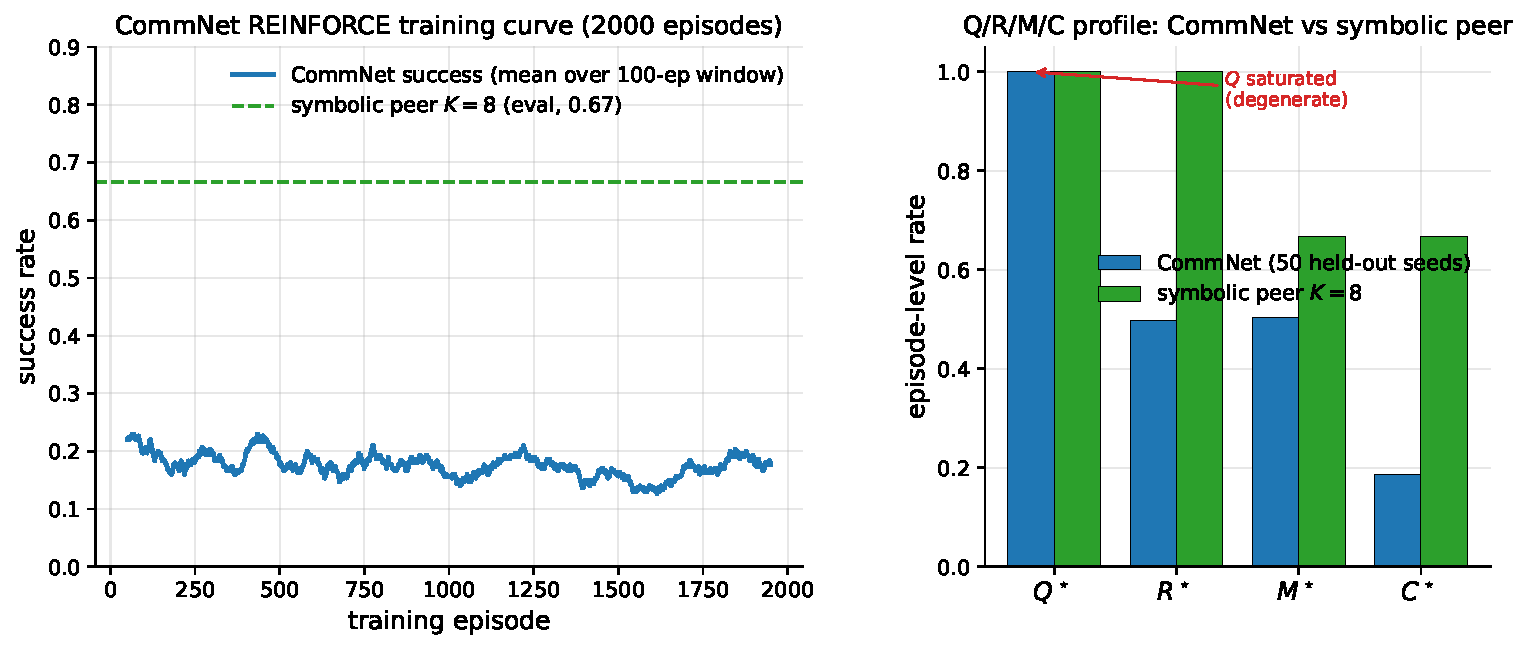
\includegraphics[width=0.95\linewidth]{figures/fig_commnet_baseline.pdf}
\caption{Диагностика базового метода обученной коммуникации. \emph{Слева:} кривая обучения CommNet (сглаженная доля успеха по окну в 100 эпизодов) за 2000 обучающих эпизодов; успех остается ниже 0.25 на всем протяжении. Пунктирная линия --- символьная одноранговая архитектура при $K\!=\!8$ на том же сценарии для сравнения. \emph{Справа:} профиль Q/R/M/C обученного CommNet на 50 отложенных сидах против символьной одноранговой при $K\!=\!8$. $Q^\star$ насыщено на уровне $1.0$ у CommNet (вырождено по построению); $R/M$ схлопываются вместе; только на символьной архитектуре условные частоты разделены.}
\label{fig:commnet}
\end{figure}

\textbf{Оценка Q/R/M/C (50 отложенных сидов, стохастическое сэмплирование действий).}

\begin{table}[h]
\centering
\small
\begin{tabular}{l c}
\toprule
Величина & Значение \\
\midrule
Частота $Q^\star$                           & \textbf{1.00} (насыщено) \\
Частота $R^\star$                           & 0.50 \\
Частота $M^\star$                           & 0.50 (схлопывается на $R$) \\
Частота $C^\star$                           & 0.19 \\
$P(R \mid Q)$                               & 0.50 \\
$P(M \mid R)$                               & 1.00 \\
$P(C \mid M)$                               & 0.42 \\
Доля успеха                                 & 0.19 \\
Среднее число шагов                         & 80 (бюджет исчерпан) \\
\bottomrule
\end{tabular}
\end{table}

Сравните с символьной одноранговой архитектурой при $K{=}8$: $P(M^\star|R^\star){=}0.69$, $P(C^\star|M^\star){=}0.87$, успех $\sim 0.65$.

\paragraph{Вариант PPO: структурная вырожденность проверена при конкурентоспособном успехе.}
Обученный PPO~\citep{schulman2017proximal} вариант той же архитектуры CommNet (clip $\epsilon{=}0.2$, обобщенная оценка преимущества~\citep{schulman2016gae} с $\lambda{=}0.95$, $\gamma{=}0.99$, 4 эпохи PPO на rollout, 64 rollout'а на обновление, 200 обновлений, $\approx 96$ минут на одном ядре CPU; полная конфигурация в \texttt{experiments/commnet\_ppo\_baseline/train\_ppo\_commnet.py}) достигает $0.667$ успеха на 100 отложенных сидах --- на уровне символьной одноранговой архитектуры при $K{=}8$ ($0.65$).

\begin{table}[h]
\centering
\small
\caption{REINFORCE против PPO CommNet против символьной одноранговой ($K{=}8$) на сценарии дефицита ($N{=}3$, $T{=}2$, асимметричная раскладка, опасность $0.05$). PPO конкурентоспособен по доле успеха, но по-прежнему демонстрирует насыщение Q и коллапс R/M --- диагностическое утверждение проверено, а не постулировано.}
\label{tab:ppo-commnet}
\begin{tabular}{l c c c}
\toprule
Метрика & CommNet REINFORCE & \textbf{CommNet PPO} & Символьная peer ($K{=}8$) \\
\midrule
Доля успеха                   & 0.19   & \textbf{0.667} & 0.65 \\
Частота $Q^\star$             & 1.00   & \textbf{1.00}  & 0.99 \\
Частота $R^\star$             & 0.50   & \textbf{0.997} & 0.69 \\
Частота $M^\star$             & 0.50   & \textbf{0.997} & 0.69 \\
$P(M^\star|R^\star)$          & 1.00   & \textbf{1.00}  & 0.69 \\
$P(C^\star|M^\star)$          & 0.42   & \textbf{0.67}  & 0.87 \\
R/M разделены?                & нет    & \textbf{нет}   & \textbf{да} \\
\bottomrule
\end{tabular}
\end{table}

Результат PPO превращает структурный аргумент из утверждения (<<бюджет обучения этого не изменил бы>>) в измерение: $Q^\star$ остается насыщенным на уровне 1.00, $P(M^\star|R^\star)$ остается 1.00 (коллапс R/M) даже при конкурентоспособном успехе. Стадия Q вырождена по построению в любой политике, чей коммуникационный канал --- вещественный вектор с обученной линейной проекцией: канал никогда не бывает информативно пустым, независимо от бюджета обучения, --- а без явного символьного интерфейса фиксации цели событие M не может отделиться от R. Только архитектуры с явным интерфейсом \emph{запроса/фиксации} (символьный стек из \S\ref{sec:archs}) раскрывают стадийно-разделимые события Q/R/M/C.

\section{Команды воспроизведения}
\label{app:repro}

Подачу сопровождает анонимизированный публичный репозиторий. Артефакты основной статьи были сгенерированы следующими скриптами; всюду предполагаются \texttt{PYTHONPATH=.} и виртуальное окружение Python 3 с \texttt{numpy}, \texttt{scipy}, \texttt{pandas}, \texttt{matplotlib}, \texttt{imageio}, \texttt{gymnasium} и \texttt{minigrid}.

\subsection*{Воспроизведение одной командой (многоагентный блок, $\approx 22$ минуты на 8 ядрах)}
\path{bash scripts/reproduce_paper.sh}

\subsection*{Одиночный агент (\S\ref{sec:validation}--\S\ref{sec:oracle})}
\begin{itemize}[leftmargin=16pt]
\item бенчмарк статьи и набор обученных базовых методов: \path{scripts/benchmark_symbolic_memory_article.py}
\item анализ статьи и генерация рисунков: \path{scripts/analyze_symbolic_memory_article.py}
\item синтетическая проверка факторизации: \path{scripts/validate_qrmc_factorization.py}
\item бенчмарк оракульных интервенций на стадиях: \path{scripts/benchmark_oracle_stage_interventions.py}
\item бенчмарк переноса на BabyAI: \path{scripts/compare_semnav_babyai.py}
\end{itemize}

\subsection*{Многоагентный случай (\S\ref{sec:multi-agent-results})}
\begin{itemize}[leftmargin=16pt]
\item Основная каденционная развертка из 25{,}920 прогонов (40 сидов, $K\le 16$, $\approx 18$ мин):
\path{python experiments/big_experiment/exp_cadence_phase.py --mode full --workers 8 --out_dir tmp/big_experiment_qrmc_40}
\item Расширенная развертка из 9{,}720 прогонов ($K\in\{32,48,64\}$, $\approx 4$ мин):
\path{python experiments/big_experiment/exp_extra_K.py --workers 8 --out_dir tmp/big_experiment_extraK}
\item Стадийный анализ Q/R/M/C и бутстреп-ДИ:
\path{python experiments/big_experiment/analyze_qrmc.py --runs_csv tmp/big_experiment_qrmc_40/runs.csv --out_dir tmp/big_experiment_qrmc_40}
\item Многоагентные оракульные интервенции:
\path{python experiments/big_experiment/exp_oracle_interventions.py --workers 8 --out_dir tmp/big_experiment_oracle}
\item Смоук-тесты фаз 1--4:
\path{python scripts/run_all_smokes.py --out_dir tmp/all_smokes}
\item Базовый метод CommNet, обученный PPO (таблица~\ref{tab:ppo-commnet}, $\approx 96$ мин на одном ядре CPU):
\path{python -m experiments.commnet_ppo_baseline.train_ppo_commnet --total_updates 200 --rollouts_per_update 64}
\item Оценка Q/R/M/C политики PPO на 100 отложенных сидах:
\path{python experiments/commnet_baseline/eval_with_qrmc.py --policy_path experiments/commnet_ppo_baseline/ppo_policy.pt --out_dir experiments/commnet_ppo_baseline --n_episodes 100}
\item Развертка переносимости на субстрате MiniGrid (\S\ref{sec:limitations}, 100 прогонов, $\approx 2$ мин):
\path{python -m experiments.minigrid_multiagent_wrapper.run_portability_sweep --out_dir tmp/minigrid_portability}
\item Бенчмарк минимальной CSM (таблица~\ref{tab:csm-results}, 3{,}240 прогонов, $\approx 5$ мин):
\path{python -m experiments.collective_semantic_memory.run_csm_benchmark --out_dir tmp/csm_benchmark}
\end{itemize}

\section{Замечание об активах и лицензиях}
\label{app:assets}

Эксперименты используют MiniGrid~\citep{MinigridMiniworld23} и BabyAI~\citep{chevalier2018babyai}, оба выпущены под лицензией MIT. Локально реализованные базовые методы и скрипты запуска бенчмарков, представленные в этой статье, будут выпущены под лицензией MIT в составе пакета артефактов camera-ready.

\clearpage
\FloatBarrier
%\input{checklist.tex}

\end{document}
